% Evaluating the Autonomous Mind: A Multi-Dimensional Framework for Agentic AI Readiness

\let\texprimitiveyear\year

\documentclass[journal,nolineno]{ieeeaccess}
\let\accessmetadatayear\year
\let\year\texprimitiveyear

% Override the IEEE Access spot color with a standard CMYK fallback for viewers
% that do not render Pantone spot colors correctly.
\definecolor{accessblue}{cmyk}{1,0.3,0,0.2}

% ── Packages ──────────────────────────────────────────────────────────
\usepackage{graphicx}
\usepackage{booktabs}
\usepackage{tabularx}
\usepackage{enumitem}
\usepackage{amsmath,amssymb}
\usepackage{xcolor}
\usepackage{tikz}
\usepackage{pgfplots}
\usepackage[numbers,sort&compress]{natbib}
\usepackage{float}
\usepackage{multicol}
\usepackage{xurl}
\usepackage{hyperref}

% ── TikZ Libraries ───────────────────────────────────────────────────
\usetikzlibrary{shapes.geometric, arrows.meta, positioning, calc, fit, backgrounds, decorations.pathreplacing, shadows.blur, matrix}

% ── pgfplots Setup ───────────────────────────────────────────────────
\pgfplotsset{compat=1.18}
\usepgfplotslibrary{polar}

% ── Colors ────────────────────────────────────────────────────────────
\definecolor{alcheblue}{RGB}{31, 78, 121}
\definecolor{alchedark}{RGB}{20, 50, 80}
\definecolor{alchegray}{RGB}{108, 117, 125}
\definecolor{alchelight}{RGB}{220, 230, 241}
\definecolor{pillar1}{RGB}{41, 128, 185}
\definecolor{pillar2}{RGB}{39, 174, 96}
\definecolor{pillar3}{RGB}{230, 126, 34}
\definecolor{pillar4}{RGB}{142, 68, 173}
\definecolor{riskred}{RGB}{192, 57, 43}
\definecolor{safegreen}{RGB}{39, 174, 96}

% ── Hyperref Setup ───────────────────────────────────────────────────
\hypersetup{
    hidelinks,
    breaklinks=true
}

% ── Custom Commands ──────────────────────────────────────────────────
\newcommand{\keyword}[1]{\textbf{#1}}

% ══════════════════════════════════════════════════════════════════════
\begin{document}

\history{Date of publication xxxx 00, 0000, date of current version April 18, 2026.}
\doi{10.1109/ACCESS.2026.XXXXXXX}

\title{Evaluating the Autonomous Mind: A Multi-Dimensional Framework for Agentic AI Readiness}

\author{Fei Wang, Salon Ren, and Eric Wang%
\thanks{Fei Wang, Salon Ren, and Eric Wang are with Alchedata AI. Corresponding author: Fei Wang.}}

\markboth{Publication Draft, April 2026}{Wang \MakeLowercase{\textit{et al.}}: Evaluating the Autonomous Mind}

\maketitle

\begin{abstract}
The transition from static large language models to autonomous agentic systems between 2024 and 2026 has exposed a fundamental measurement crisis: evaluation methodologies inherited from traditional natural language processing fail to capture the non-deterministic, multi-step, tool-mediated nature of agentic behavior. Binary success metrics treat agents as black boxes, measuring where they ended up rather than how they got there, a phenomenon described in recent literature as the \emph{success masking problem}. This paper presents a critical survey of emerging evaluation research and synthesizes the findings into an integrated conceptual framework. We organize the literature around four functional evaluation pillars (core model, memory, tool use, and environment), survey trajectory-level metrics that inspect complete execution paths, review agent-as-a-judge paradigms alongside reliability stress-testing via the Judge Reliability Harness, and examine the open-source and commercial tooling ecosystem. Drawing on this synthesis, we propose the CLEAR dimensions (cost, latency, efficacy, adherence, resilience) and Cost-Normalized Accuracy (CNA) as candidate standards for structured deployment assessment---acknowledging that neither has yet achieved formal community consensus. The paper identifies a persistent measurement imbalance that allows agents to pass benchmarks while failing in production, and offers recommendations for closing that gap. Four original synthesis contributions are introduced: a Phase--Pillar Failure Matrix that unifies failure diagnostics across cognitive phases and architectural components; a cross-benchmark coverage analysis of nine representative benchmarks revealing systematic gaps in memory, economic, adherence, and resilience coverage; an Evaluation Readiness Maturity Model (ERMM) providing a five-level diagnostic framework for practitioners; and the concept of evaluation horizon, formalizing the finite period over which a benchmark retains discriminative validity before training-data contamination degrades its signal. All quantitative claims are attributed to the primary studies that generated them and should be interpreted within the scope of those studies' evaluation setups.
\end{abstract}

\begin{IEEEkeywords}
Agent-as-a-Judge, agentic AI, Cost-Normalized Accuracy, enterprise readiness, evaluation frameworks, trajectory metrics.
\end{IEEEkeywords}

% ══════════════════════════════════════════════════════════════════════
% SECTION I
% ══════════════════════════════════════════════════════════════════════
\section{Introduction: The Death of the Black-Box Success Metric}
\label{sec:intro}

\subsection{Scope and Contributions}

This paper is a \textbf{critical survey} of evaluation frameworks for agentic AI systems, covering the research landscape from 2024 to early 2026. It does not introduce a new empirical benchmark or report original experimental results. Rather, it synthesizes findings across the literature, identifies structural gaps, and proposes a set of candidate conceptual frameworks to guide both researchers and practitioners. Specifically, our six major contributions are:

\begin{enumerate}
    \item A synthesis of the core architectural evaluation problem for agentic systems, integrating the four-pillar model (core model, memory, tool use, environment) with the broader claim that black-box outcome metrics are structurally inadequate for autonomous, multi-step behavior.
    \item A critical review of automated evaluator design, spanning LLM-as-a-Judge, Agent-as-a-Judge, judge bias taxonomies, and perturbation-based reliability testing through the Judge Reliability Harness.
    \item A consolidated diagnostic framework for failure analysis, centered on the \textbf{Phase--Pillar Failure Matrix} and related trajectory-level reasoning tools that map failure modes across cognitive phases and architectural components.
    \item Two deployment-oriented synthesis proposals for community discussion: the \textbf{CLEAR} readiness dimensions and \textbf{Cost-Normalized Accuracy (CNA)}. These are not validated standards, but structured frameworks that organize technical, operational, and economic evaluation criteria.
    \item A multi-layer analysis of the measurement gap in current practice, including the measurement imbalance thesis, a \textbf{cross-benchmark coverage analysis} (Table~\ref{tab:benchmark_coverage}) across nine representative benchmarks, and a concrete agenda for integrating human-centered, economic, and resilience metrics.
    \item Two organization-level strategy constructs for improving long-term evaluation practice: the \textbf{Evaluation Readiness Maturity Model} (ERMM) for capability development and the concept of \textbf{evaluation horizon} for reasoning about benchmark decay under training-data contamination.
\end{enumerate}

Frameworks labeled CLEAR and CNA throughout this paper are presented as conceptual syntheses and proposals. Claims about specific quantitative thresholds (e.g., alignment percentages, code-complexity limits) are attributed to the primary studies that generated them and are explicitly scoped to those studies' evaluation conditions.

\subsection{The Transition from LLM Chatbots to Agentic Collaborators}

Between 2024 and 2026, the enterprise AI landscape underwent a fundamental transformation. The shift from standard large language models to autonomous agentic systems represents not an incremental improvement in capability, but a qualitative change in the computational paradigm itself. Where traditional LLMs operated as sophisticated response engines---accepting a prompt and returning a completion---agentic systems function as persistent, goal-directed entities that perceive, plan, act, and interact with complex environments over extended timeframes.

This transition has been driven by three converging forces. First, the maturation of model capabilities---particularly in reasoning and instruction following---has made it feasible for LLMs to serve as the cognitive core of autonomous systems. Second, the development of standardized tool-use protocols and orchestration frameworks (LangChain, LangGraph, CrewAI, AutoGen) has lowered the engineering barrier to building multi-step agent workflows. Third, enterprise demand for automation that goes beyond content generation---toward actual task execution---has created a commercial imperative for agentic deployment.

The result has been a marked acceleration in production-grade agentic deployments. Chat interfaces, browser-based agents, and enterprise automation platforms have led the adoption wave. Industry surveys suggest high but not precisely verified rates of enterprise piloting~\citep{mckinsey_agentic_ai}, and documented deployments span customer service automation, software development assistance, and structured workflow execution---though the scope and autonomy of these deployments vary considerably and resist precise quantification from the academic literature alone. Autonomous agency in high-stakes domains such as financial transactions or claims processing remains nascent and typically involves significant human-in-the-loop oversight.

\subsection{Defining ``Agenticness'': Autonomy, Goal-Driven Reasoning, and Scaffolded Intelligence}

Not every system that uses an LLM is agentic. The distinction matters because the degree of agency directly determines the complexity of the evaluation challenge. We define agenticness along three axes:

\begin{description}
    \item[Autonomy] The system's capacity to generate tasks, decisions, and strategies without explicit step-by-step human instruction. A conventional AI requires predefined inputs and task boundaries; an agentic system defines its own sub-goals and execution path.
    \item[Goal-Driven Reasoning] The system's ability to decompose high-level objectives into actionable plans and pursue them across multiple steps, adapting when intermediate results deviate from expectations. This is distinct from single-turn inference, where the model responds to an isolated prompt.
    \item[Scaffolded Intelligence] The degree to which the system's capability is determined not just by the underlying model, but by the surrounding cognitive architecture: prompt engineering, reflection loops, planning layers, memory management, and tool orchestration. A critical finding from 2025 research is that even when underlying models (like GPT-4 or Claude 3.5) are older or less capable, the agentic scaffolding determines the ultimate capability and productization of the system~\citep{beyond_task_completion}.
\end{description}

These three axes define a spectrum of agenticness. A system that exhibits all three at high levels is fully agentic; one that exhibits some is semi-agentic. The evaluation methodology must scale with the degree of agency. Table~\ref{tab:conventional_vs_agentic} contrasts the two paradigms.

\begin{table}[htbp]
\centering
\caption{Conventional AI vs.\ Agentic AI across key dimensions.}
\label{tab:conventional_vs_agentic}
\resizebox{0.96\columnwidth}{!}{%
\begin{tabular}{@{}lll@{}}
\toprule
\textbf{Dimension} & \textbf{Conventional AI} & \textbf{Agentic AI} \\
\midrule
Adaptability & Predefined tasks, static rules & Dynamic, evolving environments \\
Autonomy & Predefined inputs, boundaries & Self-generated sub-goals \\
Data Dependency & Fixed training data & Real-time perception \& planning \\
Decision-Making & Deterministic rules & Context-aware, multi-agent \\
Resource Requirements & Moderate complexity & High orchestration demands \\
\bottomrule
\end{tabular}
}
\end{table}

\subsection{The Inadequacy of Current Benchmarks: Non-Determinism and the ``Success Masking'' Problem}

Traditional model evaluation is outcome-based: did the model produce the correct output given this input? For a summarization task or a classification benchmark, this is reasonable. The output is the artifact. There is nothing else to measure.

Agents are different. An agent operates in a continuous decision loop---sensing, planning, acting, and updating state across multiple turns and tool calls. The final output may be correct even when the path to it was broken: an agent can complete a task while violating a safety policy, bypassing an authorization check, or skipping a diagnostic step that would have caught a downstream failure.

Binary success metrics treat the agent as a black box. They measure where it ended up, not how it got there.

This is what researchers now call the \keyword{success masking problem}---agents that appear to succeed while simultaneously creating latent risk. It is not a corner case. It is a systematic failure mode of any evaluation methodology that ignores the execution trajectory~\citep{beyond_benchmark_islands}.

Figure~\ref{fig:success_masking} illustrates this problem: outcome-only evaluation sees only the final result, while trajectory evaluation reveals the policy violations and skipped steps along the path.

\begin{figure*}[htbp]
\centering
                    % Success Masking Problem: Outcome vs Trajectory Evaluation
\resizebox{0.96\textwidth}{!}{%
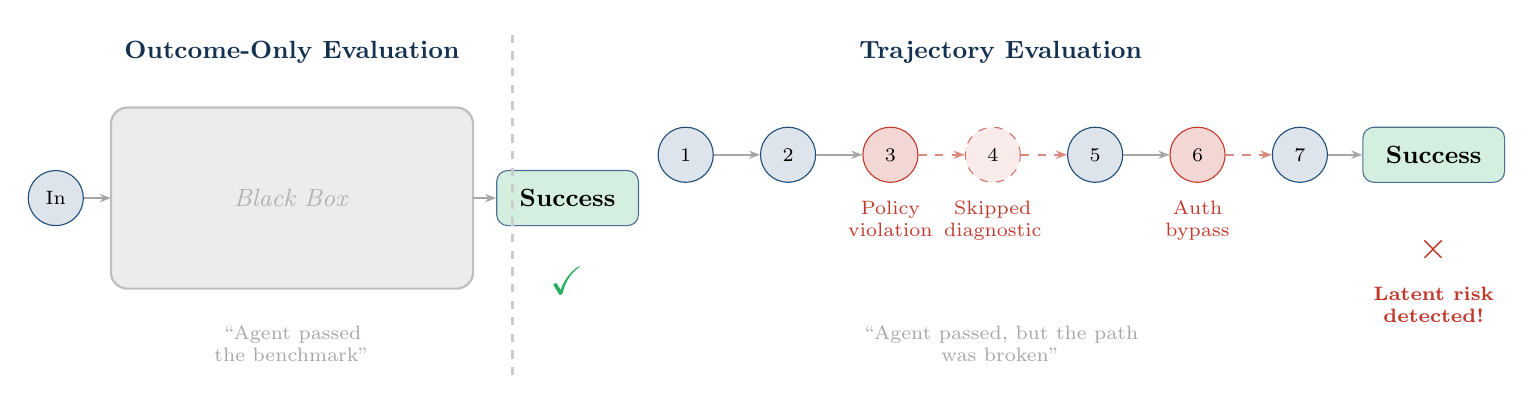
\begin{tikzpicture}[
    gstep/.style={circle, draw=alcheblue, fill=alcheblue!15, minimum size=0.7cm, font=\scriptsize, inner sep=1pt},
    badstep/.style={circle, draw=riskred, fill=riskred!20, minimum size=0.7cm, font=\scriptsize, inner sep=1pt},
    skipstep/.style={circle, draw=riskred!70, fill=riskred!10, minimum size=0.7cm, font=\scriptsize, inner sep=1pt, dashed},
    result/.style={rectangle, rounded corners=4pt, draw=alcheblue!80, fill=safegreen!20, minimum width=1.8cm, minimum height=0.7cm, font=\small\bfseries, align=center},
    badresult/.style={rectangle, rounded corners=4pt, draw=riskred!80, fill=riskred!10, minimum width=1.8cm, minimum height=0.7cm, font=\small\bfseries, align=center},
    lbl/.style={font=\small\bfseries, text=alchedark},
    ann/.style={font=\scriptsize, text=riskred, align=center},
    arr/.style={-{Stealth[length=4pt]}, thick, gray!70},
    badarr/.style={-{Stealth[length=4pt]}, thick, riskred!60, dashed}
]

% ── Left: Outcome-Only Evaluation ──
\node[lbl] at (-3.5, 3.5) {Outcome-Only Evaluation};

% Black box
\fill[gray!15, rounded corners=6pt] (-5.8, 0.5) rectangle (-1.2, 2.8);
\draw[gray!50, thick, rounded corners=6pt] (-5.8, 0.5) rectangle (-1.2, 2.8);
\node[font=\small, text=gray!60] at (-3.5, 1.65) {\textit{Black Box}};

% Input
\node[gstep] (i1) at (-6.5, 1.65) {In};
\draw[arr] (i1) -- (-5.8, 1.65);

% Output
\node[result] (o1) at (0, 1.65) {Success};
\draw[arr] (-1.2, 1.65) -- (o1);

% Checkmark
\node[font=\Large, text=safegreen] at (0, 0.6) {\checkmark};

% Label
\node[font=\scriptsize, text=gray!70, align=center] at (-3.5, -0.2) {``Agent passed\\the benchmark''};

% ── Right: Trajectory Evaluation ──
\node[lbl] at (5.5, 3.5) {Trajectory Evaluation};

% Steps
\node[gstep] (s1) at (1.5, 2.2) {1};
\node[gstep] (s2) at (2.8, 2.2) {2};
\node[badstep] (s3) at (4.1, 2.2) {3};
\node[skipstep] (s4) at (5.4, 2.2) {4};
\node[gstep] (s5) at (6.7, 2.2) {5};
\node[badstep] (s6) at (8.0, 2.2) {6};
\node[gstep] (s7) at (9.3, 2.2) {7};

% Arrows between steps
\draw[arr] (s1) -- (s2);
\draw[arr] (s2) -- (s3);
\draw[badarr] (s3) -- (s4);
\draw[badarr] (s4) -- (s5);
\draw[arr] (s5) -- (s6);
\draw[badarr] (s6) -- (s7);

% Annotations
\node[ann, below=3pt of s3] {Policy\\violation};
\node[ann, below=3pt of s4] {Skipped\\diagnostic};
\node[ann, below=3pt of s6] {Auth\\bypass};

% Result
\node[result] (o2) at (11, 2.2) {Success};
\draw[arr] (s7) -- (o2);

% But with warning
\node[font=\Large, text=riskred] at (11, 1.0) {\texttimes};
\node[font=\scriptsize\bfseries, text=riskred, align=center] at (11, 0.3) {Latent risk\\detected!};

% Label
\node[font=\scriptsize, text=gray!70, align=center] at (5.5, -0.2) {``Agent passed, but the path\\was broken''};

% Divider
\draw[gray!40, dashed, thick] (-0.7, -0.6) -- (-0.7, 3.8);

\end{tikzpicture}
}
\caption{The success masking problem. Outcome-only evaluation (left) sees only the final result, while trajectory evaluation (right) reveals policy violations and skipped steps along the execution path.}
\label{fig:success_masking}
\end{figure*}

The implications are severe. Organizations are making multi-million dollar infrastructure commitments based on evaluation methodologies that were designed for a fundamentally different paradigm. The result is a growing class of production failures that are entirely invisible to the benchmarks teams rely on.


% ══════════════════════════════════════════════════════════════════════
% SECTION II
% ══════════════════════════════════════════════════════════════════════
\section{Theoretical Foundations of Agent Assessment}
\label{sec:foundations}

\subsection{The Four-Pillar Model: Core Model, Memory, Tools, and Environment}

Effective agentic evaluation requires decomposing the agent into its functional components and testing each independently. The Agent Assessment Framework (AAF), developed from foundational work at Anthropic and refined in industry deployments, proposes four architectural pillars~\citep{beyond_task_completion}. These pillars isolate specific components of the agentic scaffold to identify where failures originate---whether in the core model, the memory system, the tool-use logic, or the environmental interaction. Figure~\ref{fig:pillar_model} provides a visual overview.

\begin{figure*}[htbp]
\centering
% Four-Pillar Model for Agent Assessment
\resizebox{0.96\textwidth}{!}{%
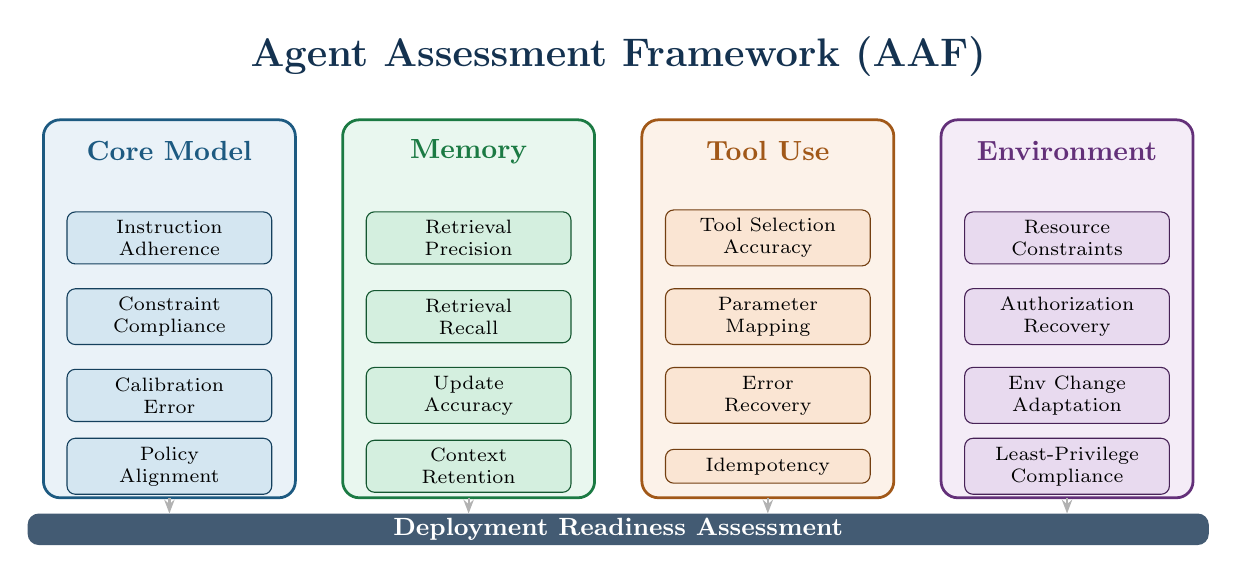
\begin{tikzpicture}[
    pillar/.style={
        rectangle, rounded corners=6pt, minimum width=3.2cm, minimum height=4.8cm,
        draw=#1!70!black, fill=#1!10, line width=1pt, align=center,
        inner sep=8pt
    },
    metric/.style={
        rectangle, rounded corners=3pt, minimum width=2.6cm,
        draw=#1!50!black, fill=#1!20, font=\scriptsize, align=center,
        inner sep=3pt
    },
    plabel/.style={font=\bfseries\normalsize, text=#1!70!black},
    arr/.style={-{Stealth[length=5pt]}, thick, color=gray!60}
]

% Pillars
\node[pillar=pillar1] (p1) at (0,0) {};
\node[pillar=pillar2] (p2) at (3.8,0) {};
\node[pillar=pillar3] (p3) at (7.6,0) {};
\node[pillar=pillar4] (p4) at (11.4,0) {};

% Pillar labels
\node[plabel=pillar1] at (0, 2.0) {Core Model};
\node[plabel=pillar2] at (3.8, 2.0) {Memory};
\node[plabel=pillar3] at (7.6, 2.0) {Tool Use};
\node[plabel=pillar4] at (11.4, 2.0) {Environment};

% Core Model metrics
\node[metric=pillar1] at (0, 0.9) {Instruction\\Adherence};
\node[metric=pillar1] at (0, -0.1) {Constraint\\Compliance};
\node[metric=pillar1] at (0, -1.1) {Calibration\\Error};
\node[metric=pillar1] at (0, -2.0) {Policy\\Alignment};

% Memory metrics
\node[metric=pillar2] at (3.8, 0.9) {Retrieval\\Precision};
\node[metric=pillar2] at (3.8, -0.1) {Retrieval\\Recall};
\node[metric=pillar2] at (3.8, -1.1) {Update\\Accuracy};
\node[metric=pillar2] at (3.8, -2.0) {Context\\Retention};

% Tool Use metrics
\node[metric=pillar3] at (7.6, 0.9) {Tool Selection\\Accuracy};
\node[metric=pillar3] at (7.6, -0.1) {Parameter\\Mapping};
\node[metric=pillar3] at (7.6, -1.1) {Error\\Recovery};
\node[metric=pillar3] at (7.6, -2.0) {Idempotency};

% Environment metrics
\node[metric=pillar4] at (11.4, 0.9) {Resource\\Constraints};
\node[metric=pillar4] at (11.4, -0.1) {Authorization\\Recovery};
\node[metric=pillar4] at (11.4, -1.1) {Env Change\\Adaptation};
\node[metric=pillar4] at (11.4, -2.0) {Least-Privilege\\Compliance};

% Top label
\node[font=\Large\bfseries, text=alchedark] at (5.7, 3.2) {Agent Assessment Framework (AAF)};

% Foundation bar
\fill[alchedark!80, rounded corners=4pt] (-1.8,-3.0) rectangle (13.2,-2.6);
\node[font=\small\bfseries, text=white] at (5.7, -2.8) {Deployment Readiness Assessment};

% Arrows from pillars to foundation
\draw[arr] (0, -2.4) -- (0, -2.6);
\draw[arr] (3.8, -2.4) -- (3.8, -2.6);
\draw[arr] (7.6, -2.4) -- (7.6, -2.6);
\draw[arr] (11.4, -2.4) -- (11.4, -2.6);

\end{tikzpicture}
}
\caption{The Four-Pillar Model for Agent Assessment. Each pillar isolates a functional component of the agentic scaffold, enabling targeted evaluation and diagnosis of failure origins.}
\label{fig:pillar_model}
\end{figure*}

\subsubsection{The Core Model Pillar}

Evaluation at the core model level focuses on instruction following and policy alignment. It assesses whether the agent adheres to the intended sequence of objectives and respects established constraints. A critical finding in 2025 research is that even when underlying models are older, the agentic scaffolding---the prompt engineering, reflection loops, and planning layers---determines the ultimate capability and productization of the system~\citep{beyond_task_completion}.

Evaluation at this pillar often involves measuring \keyword{calibration error}---the alignment between an agent's confidence and its actual accuracy---which is vital for risk-sensitive workflows. An agent that is consistently overconfident in incorrect outputs is far more dangerous than one that signals uncertainty. Calibration error is measured by comparing the agent's self-assessed confidence scores against its actual success rate across a distribution of tasks.

Key metrics for the core model pillar include:
\begin{itemize}
    \item \textbf{Instruction adherence rate}: The proportion of tasks where the agent follows the specified instruction sequence without deviation.
    \item \textbf{Constraint compliance}: Whether the agent respects boundaries established earlier in a conversation or workflow.
    \item \textbf{Calibration error}: The divergence between confidence estimates and actual accuracy, typically measured using Expected Calibration Error (ECE).
    \item \textbf{Policy alignment}: The degree to which the agent's behavior conforms to stated operational policies.
\end{itemize}

\subsubsection{The Memory Pillar}

Memory management is evaluated through storage efficiency and retrieval accuracy. This pillar measures the agent's ability to update contextual data without duplication and tracks ``update latency''---the time between an environmental change and the agent's incorporation of that change into its working context.

In long-running sessions, agents frequently suffer from \keyword{context retention failures}---losing track of constraints established in early turns, a phenomenon sometimes called being ``lost in the middle'' of the context window. This is not merely an inconvenience; in production workflows, an agent that forgets a constraint established in turn 3 can violate a safety policy in turn 15 without any awareness of the violation.

Metrics such as Precision, Recall, F1-score, and BLEU-1 are employed against gold-standard labels to ensure accurate information extraction from historical context:
\begin{itemize}
    \item \textbf{Retrieval precision}: Of the information the agent retrieved from memory, how much was relevant to the current task?
    \item \textbf{Retrieval recall}: Of the information available in memory that was relevant, how much did the agent actually retrieve?
    \item \textbf{Update accuracy}: When the agent updates its context with new information, how accurately does it represent the change?
    \item \textbf{Duplication rate}: The frequency with which the agent stores redundant or conflicting information in memory.
    \item \textbf{Context retention span}: The number of turns over which the agent maintains accurate awareness of previously established constraints.
\end{itemize}

\subsubsection{The Tool Use Pillar}

Tool interaction is perhaps the most active area of agentic failure. Evaluation frameworks assess tool selection accuracy, parameter mapping, and tool sequencing. For instance, an agent must not only choose the correct tool (e.g., a monitoring tool vs.\ an audit tool) but must also pass semantically accurate parameters, such as using an Instance ID rather than a Region Name.

Production-grade agents must demonstrate resilience by recognizing and recovering from invalid tool invocations, malformed parameters, and unexpected response formats. The tool use pillar evaluates:
\begin{itemize}
    \item \textbf{Tool selection accuracy}: Whether the agent chooses the appropriate tool for each sub-task.
    \item \textbf{Parameter mapping fidelity}: Whether the agent passes correct, semantically appropriate parameters to each tool.
    \item \textbf{Tool sequencing}: Whether the agent calls tools in the correct order when dependencies exist.
    \item \textbf{Error recovery}: The agent's ability to recognize and handle invalid invocations and malformed responses without cascading failure.
    \item \textbf{Idempotency}: Whether the agent can handle retries safely without causing unintended side effects, such as duplicating a purchase or a data entry.
\end{itemize}

\subsubsection{The Environment Pillar}

Environmental evaluation examines how the agent responds to resource limitations, authorization failures, and changes in environmental constraints. It assesses the agent's ability to preserve intended workflows within real or simulated operational contexts. Secure operation in these environments requires validating authentication, enforcing role-based access controls, and limiting agent access based on least-privilege principles.

The environment pillar is particularly important because it tests the agent's behavior under conditions that are difficult to replicate in static test sets:
\begin{itemize}
    \item \textbf{Resource constraint handling}: How the agent behaves when API rate limits are hit, memory is constrained, or compute resources are limited.
    \item \textbf{Authorization failure recovery}: Whether the agent gracefully handles permission errors and seeks alternative approaches rather than retrying indefinitely.
    \item \textbf{Environmental change adaptation}: Whether the agent detects and adapts when the environment changes.
    \item \textbf{Least-privilege compliance}: Whether the agent restricts its own actions to the minimum necessary permissions.
\end{itemize}

Testing across all four pillars is what separates a benchmark score from a deployment readiness assessment.

\subsection{Static Verification vs.\ Dynamic Execution Monitoring}

The assessment of agentic AI has moved beyond static test sets toward dynamic, interactive, and judge-based methodologies that capture the fluid nature of agent-environment interactions.

Static analysis validates agent behavior against predefined ground-truth specifications and ``golden labels.'' This approach is necessary but insufficient. It confirms that the agent produces correct outputs for known inputs, but it cannot capture the full range of behaviors that emerge during actual execution.

However, many failures in multi-agent systems only surface during dynamic execution. Dynamic analysis involves monitoring runtime behaviors to detect deviations, policy violations, and guardrail breaches during actual interaction with tools and environments. This approach allows for the measurement of \keyword{trajectory metrics}, which evaluate the complete execution path---every reasoning step and tool call---rather than just the final output.

The distinction is fundamental, as summarized in Table~\ref{tab:static_vs_dynamic}.

\begin{table}[htbp]
\centering
\caption{Static verification vs.\ dynamic execution monitoring.}
\label{tab:static_vs_dynamic}
\resizebox{0.96\columnwidth}{!}{%
\begin{tabular}{@{}lll@{}}
\toprule
\textbf{Aspect} & \textbf{Static Verification} & \textbf{Dynamic Monitoring} \\
\midrule
What is measured & Output vs.\ golden labels & Complete execution trajectory \\
When measured & Pre-deployment, curated test sets & During execution, real/simulated env \\
Failure modes & Incorrect outputs & Process failures, policy violations \\
Adaptability & Fixed test set & Responsive to env changes \\
Scalability & High (automated) & Moderate (requires instrumentation) \\
Coverage & Known scenarios & Emergent behaviors \\
\bottomrule
\end{tabular}
}
\end{table}

Effective evaluation requires both. Static verification provides a baseline; dynamic monitoring reveals the behaviors that matter in production.

\subsection{The Socio-Technical Scenario Manifold: Beyond Benchmark Islands}

A fundamental limitation of current evaluation practice is its reliance on what researchers call ``benchmark islands''---disconnected instances of task completion that fail to represent the full distribution of conditions an agent will encounter in deployment.

The Holographic Agent Assessment Framework (HAAF) proposes a move from benchmark islands to a \keyword{scenario manifold} that characterizes agent trustworthiness over a representative socio-technical distribution~\citep{beyond_benchmark_islands}. The framework models each scenario $s \in \mathcal{S}$ as a structured configuration varying along axes such as task objective, tool interface, and social context. The framework produces a vector of trustworthiness measurements $\mathbf{m}(a, s)$, which are then aggregated over a weighted test set $Q \subset \mathcal{S}$ to yield an estimated trustworthiness profile:
\begin{equation}
    \hat{\mathbf{T}}_Q(a) = \frac{1}{Z} \sum_{s \in Q} w(s)\, \mathbf{m}(a, s)
\end{equation}
where $w(s)$ encodes deployment relevance and risk sensitivity, and $Z$ is a normalization factor. This allows for a risk-aware assessment where high-consequence scenarios are upweighted.

The key insight is that not all scenarios are equally important. An agent that performs well on low-stakes tasks but fails on high-stakes ones is not trustworthy, even if its average performance across all scenarios appears acceptable. The scenario manifold approach enables organizations to weight evaluation by the consequences of failure, producing an assessment that reflects real-world risk.

This represents a paradigm shift from ``how often does the agent succeed?'' to ``how trustworthy is the agent in the scenarios that matter most?''


% ══════════════════════════════════════════════════════════════════════
% SECTIONS III–IX (loaded from sub-files)
% ══════════════════════════════════════════════════════════════════════
% ══════════════════════════════════════════════════════════════════════
% SECTION III
% ══════════════════════════════════════════════════════════════════════
\section{Cognitive Diagnostics: Probing the Reasoning Trace}
\label{sec:cognitive}

\subsection{Repository-Level Reasoning and the Aggregation Deficit}

As agentic systems are deployed on increasingly complex tasks---particularly in software engineering---evaluation must probe not just whether the agent produces correct output, but whether it can reason effectively about large, interdependent code systems.

RepoReason is a diagnostic benchmark designed to evaluate repository-level reasoning in LLM agents~\citep{agent_gpa}. It moves away from code generation to a \keyword{verification-centric} approach called Abductive Assertion Verification. By masking unit test assertions and requiring the model to derive values that satisfy them, RepoReason tests the agent's ability to mentally reconstruct execution history across massive, interdependent file systems.

This approach is significant because it directly tests the kind of reasoning that production agents must perform: understanding how changes in one file propagate through dependencies, predicting the behavior of code without executing it, and synthesizing information across multiple modules.

Findings from RepoReason have identified critical performance ceilings for current frontier models that have direct implications for deployment:

\begin{description}[style=nextline,leftmargin=1em]
    \item[The Cliff Effect] Reading comprehension accuracy drops sharply when the volume of code exceeds approximately 600 lines. This is not a gradual decline but a precipitous drop---agents that perform well on 500-line codebases may fail catastrophically on 700-line ones.
    \item[The Aggregation Deficit] Accuracy declines as ``integration width'' increases---meaning the number of cross-file dependencies the agent must synthesize. This is precisely the condition that characterizes real production codebases, where changes in one module can affect behavior in seemingly unrelated components.
    \item[Consistency Decay] Models show a significant loss of consistency beyond 100 execution steps in a single trajectory. An agent that reasons correctly in steps 1--80 may begin making errors in steps 80--120, not because the later steps are harder, but because the accumulated context degrades the agent's reasoning coherence.
\end{description}

These are not model-specific quirks. They reflect fundamental constraints on how current architectures handle deep, multi-file reasoning at scale. Any evaluation methodology that does not test for these failure modes will produce overconfident deployment assessments.

\subsection{The ``Cliff Effect'' and Simulation Depth Limits}

The Cliff Effect deserves particular attention because it represents a qualitative rather than quantitative failure mode. Unlike gradual performance degradation, the Cliff Effect means that an agent can appear fully competent right up to the point where it catastrophically fails.

This has profound implications for evaluation:

\begin{enumerate}[nosep]
    \item \textbf{Interpolation is dangerous.} If an agent performs well on 400-line codebases and poorly on 800-line ones, it is not safe to assume it performs acceptably on 600-line codebases. The cliff may occur at any point.
    \item \textbf{Benchmark results can be misleading.} A benchmark that uses 500-line codebases will produce optimistic results that do not generalize to the 700+ line codebases common in production.
    \item \textbf{Safety margins must be explicit.} Organizations must define maximum complexity thresholds for their agents and enforce them in production, rather than discovering the cliff through failures.
\end{enumerate}

The simulation depth limit---the point at which an agent's reasoning coherence degrades beyond recovery---is similarly consequential. For agents operating in multi-turn workflows, the 100-step consistency decay means that long-running tasks are inherently less reliable than short ones. This must be accounted for in both evaluation and deployment design:
\begin{itemize}[nosep]
    \item Break long workflows into shorter segments with verification checkpoints.
    \item Implement intermediate validation steps that can catch reasoning drift before it compounds.
    \item Monitor trajectory coherence in real-time and escalate to human oversight when degradation is detected.
\end{itemize}

\subsection{Agent GPA: Decomposing the Goal-Plan-Action Cycle}

Traditional evaluation treats task completion as a monolithic outcome. But agentic behavior can be decomposed into three distinct cognitive phases, each of which can fail independently~\citep{agent_gpa}:

\begin{enumerate}[nosep]
    \item \textbf{Goal comprehension}: Does the agent correctly understand what it is being asked to do?
    \item \textbf{Plan formulation}: Does the agent devise a sensible strategy for achieving the goal?
    \item \textbf{Action execution}: Does the agent correctly implement the plan through tool calls and environmental interactions?
\end{enumerate}

The \keyword{Agent GPA} (Goal-Plan-Action) framework evaluates each phase independently, producing a profile rather than a single score. Figure~\ref{fig:agent_gpa} illustrates this decomposition.

\begin{figure}[htbp]
\centering
% Agent GPA: Goal-Plan-Action Alignment Framework
\resizebox{\textwidth}{!}{%
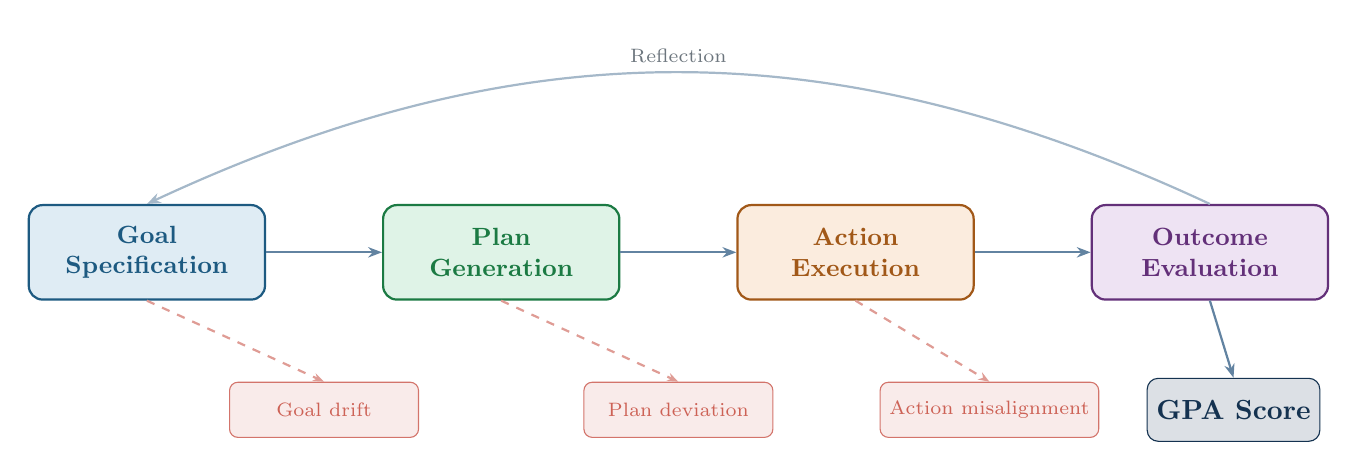
\begin{tikzpicture}[
    box/.style={rectangle, rounded corners=5pt, draw=#1!70!black, fill=#1!15, 
        minimum width=3cm, minimum height=1.2cm, align=center, font=\small\bfseries, 
        text=#1!70!black, line width=0.8pt},
    fail/.style={rectangle, rounded corners=3pt, draw=riskred!70, fill=riskred!10,
        minimum width=2.4cm, minimum height=0.7cm, align=center, font=\scriptsize,
        text=riskred!80},
    arr/.style={-{Stealth[length=5pt]}, thick, alcheblue!70},
    farr/.style={-{Stealth[length=4pt]}, thick, riskred!50, dashed}
]

% Main pipeline
\node[box=pillar1] (goal) at (0,0) {Goal\\Specification};
\node[box=pillar2] (plan) at (4.5,0) {Plan\\Generation};
\node[box=pillar3] (action) at (9,0) {Action\\Execution};
\node[box=pillar4] (result) at (13.5,0) {Outcome\\Evaluation};

% Arrows
\draw[arr] (goal) -- (plan);
\draw[arr] (plan) -- (action);
\draw[arr] (action) -- (result);

% Failure modes below
\node[fail] (f1) at (2.25,-2) {Goal drift};
\node[fail] (f2) at (6.75,-2) {Plan deviation};
\node[fail] (f3) at (10.7,-2) {Action misalignment};

\draw[farr] (goal.south) -- (f1.north);
\draw[farr] (plan.south) -- (f2.north);
\draw[farr] (action.south) -- (f3.north);

% GPA score
\node[rectangle, rounded corners=4pt, draw=alchedark, fill=alchedark!15, 
    minimum width=2cm, minimum height=0.8cm, font=\bfseries, text=alchedark] 
    (gpa) at (13.8,-2) {GPA Score};
\draw[arr] (result.south) -- (gpa.north);

% Feedback loop
\draw[arr, bend right=25, alcheblue!40] (result.north) to node[above, font=\scriptsize, text=alchegray] {Reflection} (goal.north);

\end{tikzpicture}
}
\caption{The Agent GPA framework decomposes agentic behavior into Goal comprehension, Plan formulation, and Action execution, with failure modes identified at each phase and a composite GPA score reflecting overall alignment.}
\label{fig:agent_gpa}
\end{figure}

This decomposition is critical because the remediation for each type of failure is fundamentally different, as shown in Table~\ref{tab:gpa_failures}.

\begin{table}[htbp]
\centering
\caption{GPA failure phases, symptoms, root causes, and remediations.}
\label{tab:gpa_failures}
\begin{tabular}{@{}llll@{}}
\toprule
\textbf{Phase} & \textbf{Symptom} & \textbf{Root Cause} & \textbf{Remediation} \\
\midrule
Goal & Solves wrong problem & Misunderstood intent & Prompt eng., clarification \\
Plan & Suboptimal path & Insufficient reasoning & Reflection loops, verification \\
Action & Execution errors & Tool use failures & Better descriptions, validation \\
\bottomrule
\end{tabular}
\end{table}

An agent with a high Goal score but low Action score understands what to do but cannot execute it. An agent with a high Action score but low Goal score can execute flawlessly---but on the wrong task. These are fundamentally different problems requiring fundamentally different solutions.
% ══════════════════════════════════════════════════════════════════════
% SECTION IV
% ══════════════════════════════════════════════════════════════════════
\section{The Evaluator Paradox: Reliability in Automated Judgment}
\label{sec:evaluator}

\subsection{LLM-as-a-Judge vs.\ Agent-as-a-Judge: Hierarchical vs.\ Monolithic Assessment}

As tasks become more open-ended and nuanced, Large Language Models are increasingly used as evaluators to assess qualities like helpfulness, coherence, and faithfulness that resist mechanical checking. This is a practical necessity---human labeling at evaluation scale is not viable for most organizations.

This is typically implemented in two paradigms:

\keyword{LLM-as-a-Judge} employs a monolithic model to perform a single-pass qualitative assessment of execution logs and outputs using structured prompts and rubrics~\citep{agent_as_judge_survey}. It is fast, scalable, and relatively inexpensive. However, it is limited by the judge's ability to process complex, multi-step execution traces in a single inference pass, and it is susceptible to systematic biases.

\keyword{Agent-as-a-Judge} employs a specialized ``auditor agent'' or decentralized team of agents that evaluates a subject agent using tool calls, code execution, and environment interaction rather than linguistic plausibility alone~\citep{agent_as_judge_icml}. The auditor agent can decompose complex evaluation goals into sub-tasks, verify claims through actual execution, and provide fine-grained feedback on specific steps in the execution trace.

Research published in 2026 demonstrates that Agent-as-a-Judge aligns with human experts approximately \textbf{90\% of the time}, significantly outperforming the \textbf{70\% alignment rate} of traditional LLM-as-a-Judge methods. The gap is explained by the auditor agent's ability to decompose complex evaluation goals into sub-tasks and verify claims through actual execution. Figure~\ref{fig:judge_comparison} contrasts the two paradigms.

\begin{figure}[htbp]
\centering
% LLM-as-a-Judge vs Agent-as-a-Judge Comparison
\resizebox{0.98\columnwidth}{!}{%
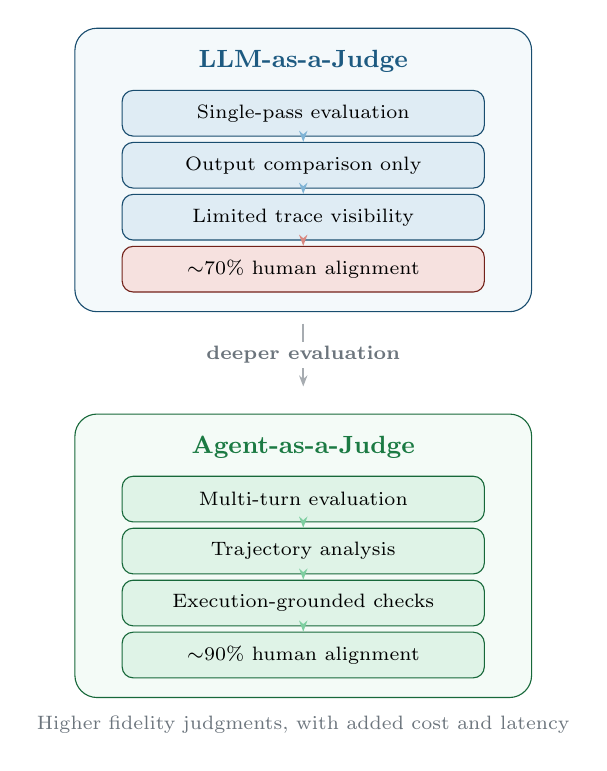
\begin{tikzpicture}[
    panel/.style={rectangle, rounded corners=8pt, draw=#1!60!black, fill=#1!5,
        minimum width=5.8cm, minimum height=3.6cm, inner sep=8pt},
    jbox/.style={rectangle, rounded corners=4pt, draw=#1!60!black, fill=#1!15,
        minimum width=4.6cm, minimum height=0.58cm, align=center, font=\scriptsize},
    arr/.style={-{Stealth[length=4pt]}, semithick, #1!60}
]

% Top panel: LLM-as-a-Judge
\node[panel=pillar1] at (0,0) {};
\node[font=\bfseries\small, text=pillar1!70!black] at (0, 1.38) {LLM-as-a-Judge};

\node[jbox=pillar1] (l1) at (0, 0.72) {Single-pass evaluation};
\node[jbox=pillar1] (l2) at (0, 0.06) {Output comparison only};
\node[jbox=pillar1] (l3) at (0, -0.60) {Limited trace visibility};
\node[jbox=riskred] (l4) at (0, -1.26) {${\sim}70\%$ human alignment};

\draw[arr=pillar1] (l1) -- (l2);
\draw[arr=pillar1] (l2) -- (l3);
\draw[arr=riskred] (l3) -- (l4);

% Middle transition
\draw[arr=alchegray] (0, -1.95) -- (0, -2.75);
\node[font=\bfseries\scriptsize, text=alchegray, fill=white, inner sep=1.5pt] at (0, -2.35) {deeper evaluation};

% Bottom panel: Agent-as-a-Judge
\node[panel=pillar2] at (0,-4.9) {};
\node[font=\bfseries\small, text=pillar2!70!black] at (0, -3.52) {Agent-as-a-Judge};

\node[jbox=pillar2] (r1) at (0, -4.18) {Multi-turn evaluation};
\node[jbox=pillar2] (r2) at (0, -4.84) {Trajectory analysis};
\node[jbox=pillar2] (r3) at (0, -5.50) {Execution-grounded checks};
\node[jbox=safegreen] (r4) at (0, -6.16) {${\sim}90\%$ human alignment};

\draw[arr=pillar2] (r1) -- (r2);
\draw[arr=pillar2] (r2) -- (r3);
\draw[arr=safegreen] (r3) -- (r4);

% Bottom annotation
\node[font=\scriptsize, text=alchegray, align=center] at (0, -7.05) {Higher fidelity judgments, with added cost and latency};

\end{tikzpicture}
}
\caption{LLM-as-a-Judge vs.\ Agent-as-a-Judge comparison. Agent-as-a-Judge provides deeper process evaluation through multi-turn analysis and trajectory inspection, achieving significantly higher human alignment.}
\label{fig:judge_comparison}
\end{figure}

The key differences are summarized in Table~\ref{tab:judge_comparison}.

\begin{table}[htbp]
\centering
\caption{LLM-as-a-Judge vs.\ Agent-as-a-Judge across key dimensions.}
\label{tab:judge_comparison}
\begin{tabular}{@{}lll@{}}
\toprule
\textbf{Feature} & \textbf{LLM-as-a-Judge} & \textbf{Agent-as-a-Judge} \\
\midrule
Evaluation Mode & Single-pass inference & Autonomous, hierarchical \\
Verification Basis & Linguistic plausibility & Execution \& interaction \\
Robustness & Prone to parametric biases & Decentralized deliberation \\
Intermediate Feedback & Limited or absent & Rich step-level feedback \\
Human Alignment & ${\sim}70\%$ & ${\sim}90\%$ \\
Cost & Lower & Higher \\
Latency & Faster & Slower \\
\bottomrule
\end{tabular}
\end{table}

The Agent-as-a-Judge paradigm addresses the cognitive overload faced by monolithic judges when assessing multi-step, complex tasks. By decomposing evaluation goals into sub-tasks and utilizing tools like code interpreters to verify the agent's actions, agentic judges can provide much finer-grained feedback and pinpoint specific flaws that might be obscured in a global score.

For production-critical workflows, the question is not just ``what did the agent do?'' but ``can we trust the system that's checking what the agent did?''

\subsection{Taxonomy of Judge Biases: Verbosity, Family, and Position Biases}

LLM judges introduce their own failure modes, and these must be understood and mitigated for evaluation results to be trustworthy. Research from the Judge Reliability Harness (JRH) identifies several systematic biases~\citep{judge_reliability_harness}:

\keyword{Verbosity Bias} --- Judges over-reward longer responses independent of quality. An agent that produces a verbose, meandering response may receive a higher score than one that produces a concise, accurate answer. This bias is particularly dangerous because it creates a perverse incentive: agents optimized against verbose judges will learn to pad their outputs, increasing token costs without improving quality.

\keyword{Position Bias} --- Judges favor responses appearing earlier in a comparison. When evaluating multiple agent outputs side by side, the judge systematically prefers the first option presented, regardless of actual quality. This bias undermines the validity of comparative evaluations and leaderboard-style rankings.

\keyword{Family Bias} --- Judges favor outputs from the same model provider. A GPT-based judge may systematically prefer GPT-generated outputs, and a Claude-based judge may prefer Claude-generated outputs. This creates a conflict of interest when the judge and the agent share the same model family.

\keyword{Format Sensitivity} --- Formatting changes produce larger reliability drops than semantic ones. A judge may assign different scores to substantively identical outputs that differ only in formatting (bullet points vs.\ paragraphs, markdown vs.\ plain text). This means that evaluation results can be manipulated by formatting choices rather than quality improvements.

These biases are not theoretical. They have been empirically demonstrated across multiple judge models and evaluation contexts. Any organization using LLM-based evaluation must account for them.

\subsection{The Judge Reliability Harness: Perturbation-Based Stress Testing}

The Judge Reliability Harness (JRH) is an open-source library developed to stress-test LLM evaluators~\citep{judge_reliability_harness}. It generates reliability tests using various perturbations to quantify how much a judge's scores should actually be trusted.

JRH employs four perturbation strategies:

\keyword{Label Flip} --- Rewriting responses to clearly violate rubrics to test discriminative accuracy. If a judge cannot reliably identify a response that has been deliberately modified to violate the evaluation criteria, the judge's discriminative ability is questionable.

\keyword{Format Invariance} --- Altering visual layouts and formatting to ensure the judge is not distracted by non-semantic changes. A reliable judge should assign the same score to substantively identical content regardless of formatting.

\keyword{Semantic Paraphrase} --- Changing wording while maintaining meaning to test scoring stability. If a judge assigns significantly different scores to paraphrased versions of the same content, the judge is evaluating surface form rather than substance.

\keyword{Verbosity Bias Tests} --- Testing whether judges over-reward longer answers when quality is held constant. By presenting the same content at different levels of verbosity, JRH can quantify the magnitude of verbosity bias.

Experiments with JRH indicate that formatting perturbations often produce larger reliability drops than semantic ones, and that judge performance in free-response tasks does not necessarily generalize to agentic settings. This is a critical finding: a judge that performs reliably on traditional NLP benchmarks may be unreliable when evaluating agentic behavior.

\textbf{Recommendations for practitioners:}

\begin{enumerate}[nosep]
    \item \textbf{Stress-test your judges before trusting them.} Run JRH-style perturbations against any LLM judge before relying on its outputs for production decisions.
    \item \textbf{Use multiple judges for high-stakes evaluations.} Employ 2--3 different judge models and require consensus or majority agreement.
    \item \textbf{Calibrate against human judgments.} Before deploying LLM-as-judge at scale, calibrate it against human evaluations on at least 100 examples.
    \item \textbf{Separate evaluation from generation.} Never use the same model to both generate agent behavior and evaluate it.
    \item \textbf{Implement judge auditing.} Regularly sample and review judge evaluations to detect drift, bias, or degradation.
\end{enumerate}
% ══════════════════════════════════════════════════════════════════════
% SECTION V
% ══════════════════════════════════════════════════════════════════════
\section{Operationalizing Agency: Economics, Safety, and Latency}
\label{sec:operational}

\subsection{The Unreliability Tax and the Cost of Autonomy}

Agentic AI introduces a fundamentally different cost model from traditional software infrastructure. Infrastructure costs are relatively fixed; intelligence costs are variable and correlated with agent complexity. When agents fail and retry, costs compound quickly.

Research into the \keyword{Unreliability Tax} identifies the additional compute, latency, and engineering required to compensate for agent failures~\citep{measurement_imbalance}. For instance, a ``Reflexion'' loop that runs for 10 cycles can consume \textbf{50 times the tokens} of a single linear pass. This is not a marginal increase---it represents a qualitative change in the economics of AI deployment.

The Unreliability Tax manifests in several ways:

\begin{itemize}
    \item \textbf{Retry costs}: When agents fail, they must retry, consuming additional tokens and API calls. In complex workflows, a single failure can trigger a cascade of retries across multiple steps.
    \item \textbf{Guardrail costs}: Implementing safety checks, validation steps, and human-in-the-loop checkpoints adds latency and token consumption to every workflow.
    \item \textbf{Observability costs}: Capturing and storing execution traces for evaluation and debugging requires infrastructure and storage.
    \item \textbf{Engineering costs}: Building and maintaining the evaluation infrastructure, red teaming pipelines, and monitoring systems represents a significant ongoing investment.
\end{itemize}

These costs are often invisible in benchmark evaluations, which typically measure accuracy in isolation. In production, they can be the difference between a viable product and an economic failure.

\subsection{CNA (Cost-Normalized Accuracy) as a New Industry Standard}

To evaluate economic efficiency, the metric of \keyword{Cost-Normalized Accuracy (CNA)} is used~\citep{beyond_accuracy}:
\begin{equation}
    \text{CNA} = \frac{\text{Accuracy}}{\text{Cost}} \times 100
\end{equation}
where Cost is measured in USD per task. CNA makes the accuracy-cost tradeoff explicit, enabling organizations to compare agents not just on how well they perform, but on how efficiently they achieve that performance.

Evaluation of leading agent architectures on enterprise tasks demonstrates a striking result, shown in Table~\ref{tab:cna_results} and visualized in Figure~\ref{fig:cna_comparison}.

\begin{table}[htbp]
\centering
\caption{Architecture comparison: efficacy, cost, and CNA.}
\label{tab:cna_results}
\resizebox{0.96\columnwidth}{!}{%
\begin{tabular}{@{}lccc@{}}
\toprule
\textbf{Architecture} & \textbf{Efficacy (\%)} & \textbf{Cost (USD/Task)} & \textbf{CNA} \\
\midrule
ReAct-GPT-o3 & 68.7 & 0.85 & 80.8 \\
Reflexion & 74.1 & 4.35 & 17.0 \\
Domain-Tuned & 81.5 & 0.31 & 260.4 \\
Plan-Execute & 71.9 & 1.05 & 68.5 \\
\bottomrule
\end{tabular}
}
\end{table}

\begin{figure*}[htbp]
\centering
% Cost-Normalized Accuracy Comparison Across Architectures
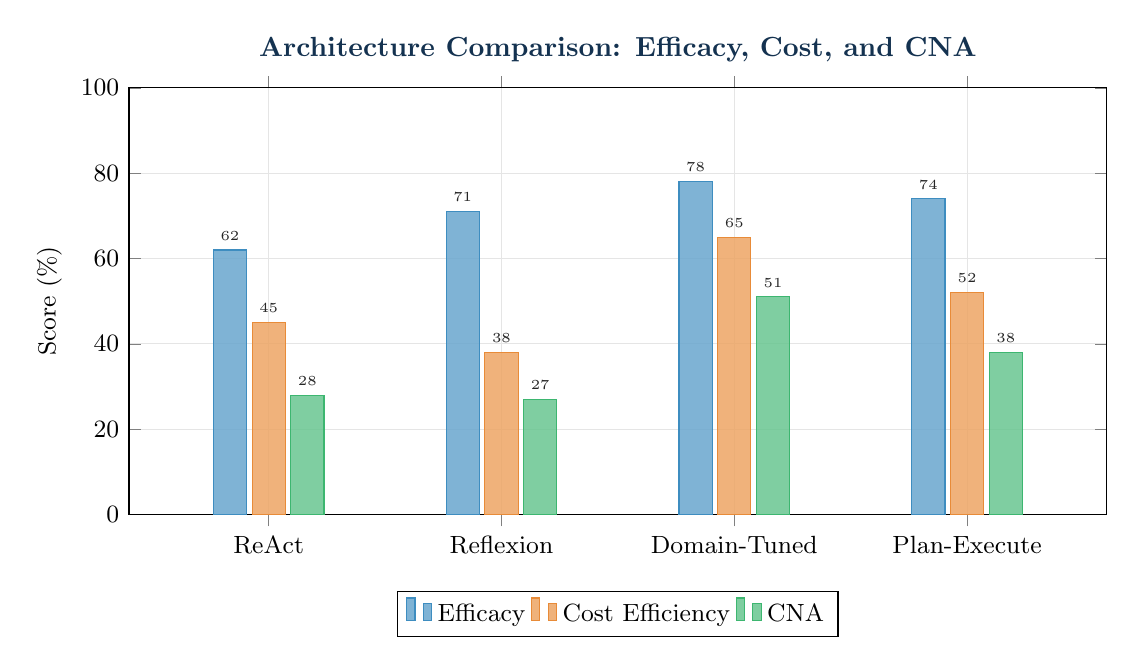
\begin{tikzpicture}
\begin{axis}[
    ybar,
    width=14cm, height=7cm,
    bar width=12pt,
    ylabel={Score (\%)},
    ylabel style={font=\small},
    symbolic x coords={ReAct, Reflexion, Domain-Tuned, Plan-Execute},
    xtick=data,
    xticklabel style={font=\small},
    yticklabel style={font=\small},
    ymin=0, ymax=100,
    legend style={at={(0.5,-0.18)}, anchor=north, legend columns=3, font=\small},
    enlarge x limits=0.2,
    nodes near coords,
    nodes near coords style={font=\tiny},
    every axis plot/.append style={fill opacity=0.85},
    grid=major,
    grid style={gray!20},
    title={\textbf{Architecture Comparison: Efficacy, Cost, and CNA}},
    title style={font=\normalsize, text=alchedark}
]

% Efficacy (task success rate)
\addplot[fill=pillar1!70, draw=pillar1!90] coordinates {
    (ReAct, 62) (Reflexion, 71) (Domain-Tuned, 78) (Plan-Execute, 74)
};

% Cost efficiency (inverse of relative cost, normalized)
\addplot[fill=pillar3!70, draw=pillar3!90] coordinates {
    (ReAct, 45) (Reflexion, 38) (Domain-Tuned, 65) (Plan-Execute, 52)
};

% CNA (cost-normalized accuracy)
\addplot[fill=pillar2!70, draw=pillar2!90] coordinates {
    (ReAct, 28) (Reflexion, 27) (Domain-Tuned, 51) (Plan-Execute, 38)
};

\legend{Efficacy, Cost Efficiency, CNA}
\end{axis}
\end{tikzpicture}
\caption{Architecture comparison across efficacy, cost efficiency, and Cost-Normalized Accuracy (CNA). The Domain-Tuned architecture achieves the highest CNA by combining strong efficacy with low cost, while Reflexion's high efficacy is undermined by excessive cost.}
\label{fig:cna_comparison}
\end{figure*}

The Reflexion architecture---often cited for its high accuracy---is \textbf{4.7$\times$ more expensive} than the domain-tuned alternative while delivering lower accuracy. The Domain-Tuned agent achieves the highest accuracy at the lowest cost, producing a CNA more than 15$\times$ higher than Reflexion.

This finding highlights what researchers call a \keyword{distorted research landscape} where expensive and fragile solutions appear superior in standard accuracy-only benchmarks~\citep{measurement_imbalance}. Simple baseline strategies can sometimes outperform complex agents at 50$\times$ lower cost.

\textbf{CNA should be a standard reporting requirement alongside any accuracy metric.} Any benchmark result reported without cost normalization is incomplete. The most accurate agent in an evaluation suite may be economically inviable at production scale.

\subsection{Security Challenges: Offensive Agentic Risk and API/MCP Gateways}

As agentic systems gain the ability to take autonomous actions, the security implications become critical~\citep{securing_ai_agents}. The attack surface of agentic environments maps across four layers, as illustrated in Figure~\ref{fig:security_layers}.

\begin{figure*}[htbp]
\centering
% Security Attack Surface: Four Layers of Agentic AI Vulnerability
\resizebox{0.96\textwidth}{!}{%
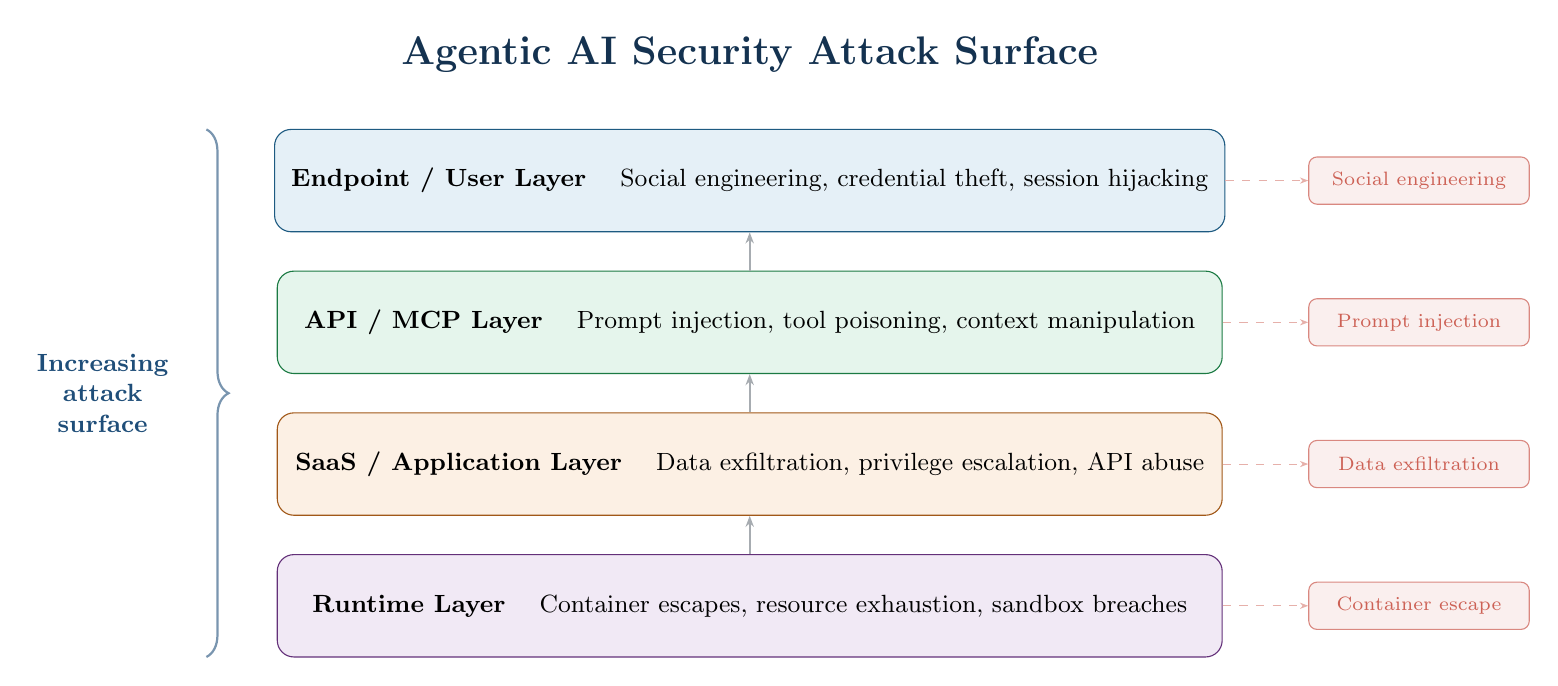
\begin{tikzpicture}[
    layer/.style={rectangle, rounded corners=6pt, draw=#1!70!black, fill=#1!12,
        minimum width=12cm, minimum height=1.3cm, align=center, font=\small,
        inner sep=6pt},
    threat/.style={rectangle, rounded corners=3pt, draw=riskred!60, fill=riskred!8,
        minimum width=2.8cm, minimum height=0.6cm, align=center, font=\scriptsize,
        text=riskred!80},
    arr/.style={-{Stealth[length=4pt]}, thick, alchegray!60}
]

% Layers (bottom to top)
\node[layer=pillar4] (l1) at (0, 0) {\textbf{Runtime Layer} \quad Container escapes, resource exhaustion, sandbox breaches};
\node[layer=pillar3] (l2) at (0, 1.8) {\textbf{SaaS / Application Layer} \quad Data exfiltration, privilege escalation, API abuse};
\node[layer=pillar2] (l3) at (0, 3.6) {\textbf{API / MCP Layer} \quad Prompt injection, tool poisoning, context manipulation};
\node[layer=pillar1] (l4) at (0, 5.4) {\textbf{Endpoint / User Layer} \quad Social engineering, credential theft, session hijacking};

% Arrows between layers
\draw[arr] (l1) -- (l2);
\draw[arr] (l2) -- (l3);
\draw[arr] (l3) -- (l4);

% Threat examples on the right
\node[threat] (t1) at (8.5, 0) {Container escape};
\node[threat] (t2) at (8.5, 1.8) {Data exfiltration};
\node[threat] (t3) at (8.5, 3.6) {Prompt injection};
\node[threat] (t4) at (8.5, 5.4) {Social engineering};

\draw[riskred!40, dashed, -{Stealth[length=3pt]}] (l1.east) -- (t1.west);
\draw[riskred!40, dashed, -{Stealth[length=3pt]}] (l2.east) -- (t2.west);
\draw[riskred!40, dashed, -{Stealth[length=3pt]}] (l3.east) -- (t3.west);
\draw[riskred!40, dashed, -{Stealth[length=3pt]}] (l4.east) -- (t4.west);

% Title
\node[font=\Large\bfseries, text=alchedark] at (0, 7.0) {Agentic AI Security Attack Surface};

% Left brace with label
\draw[decorate, decoration={brace, amplitude=8pt, mirror}, thick, alcheblue!60]
    (-6.9, -0.65) -- (-6.9, 6.05)
    node[midway, left=10pt, font=\small\bfseries, text=alcheblue, align=center] {Increasing\\attack\\surface};

\end{tikzpicture}
}
\caption{The four-layer security attack surface for agentic AI systems, from runtime infrastructure to endpoint users, with representative threat vectors at each layer.}
\label{fig:security_layers}
\end{figure*}

\begin{enumerate}
    \item \textbf{The Endpoint Layer} (e.g., coding agents): Compromise of the agent's execution environment, including local file systems, development environments, and developer machines.
    \item \textbf{The API/MCP Gateway Layer} (tool exchanges): Manipulation of the tool interfaces that agents use to interact with external systems. A compromised API can feed the agent malicious data, causing it to take harmful actions.
    \item \textbf{The SaaS Platform Layer}: Exploitation of the SaaS applications that agents interact with---CRM systems, communication platforms, cloud services---through the agent's authorized access.
    \item \textbf{The Runtime Layer}: Attacks on the agent's execution runtime, including prompt injection, context manipulation, and goal hijacking.
\end{enumerate}

CISOs are encouraged to implement a three-stage security framework:

\begin{itemize}
    \item \textbf{Visibility}: Knowing what agents you have, what tools they can access, and what actions they are taking. You cannot secure what you cannot see.
    \item \textbf{Configuration}: Reducing the blast radius by implementing least-privilege access, tool restrictions, and action boundaries. Agents should have the minimum permissions necessary for their tasks.
    \item \textbf{Runtime Protection}: Monitoring agent behavior in real-time for anomalous actions, policy violations, and indicators of compromise.
\end{itemize}

The security challenge is compounded by the fact that agentic systems can be manipulated through their inputs in ways that traditional software cannot. Prompt injection---embedding malicious instructions in data that the agent processes---can cause agents to take actions that violate their intended behavior. Tool poisoning---manipulating the outputs of tools that the agent relies on---can cause agents to make incorrect decisions based on falsified information.

These security considerations must be integrated into evaluation from the beginning, not bolted on after deployment. An evaluation framework that does not test for security vulnerabilities is providing a false sense of security.
% ══════════════════════════════════════════════════════════════════════
% SECTION VI
% ══════════════════════════════════════════════════════════════════════
\section{From Lab to Production: The Enterprise Readiness Standard}
\label{sec:enterprise}

\subsection{The CLEAR Framework for Deployment Governance}

Moving from pilots to production-grade deployment requires holistic evaluation across multiple dimensions simultaneously. Drawing on the multi-dimensional framework proposed by \citet{beyond_accuracy} and corroborated by practitioner reports~\citep{aws_evaluating_agents, production_ready_agentic}, we synthesize and name five recurring evaluation dimensions as the \keyword{CLEAR framework}. CLEAR is a conceptual synthesis proposed in this survey to organize the deployment-readiness criteria that appear most consistently across the literature; it is not yet an established industry standard or a formally validated assessment instrument. The five dimensions are:

\begin{description}
    \item[C --- Cost per task] (absolute and normalized): Not just the raw cost of API calls and compute, but the cost normalized by task complexity and success rate. CNA provides the standard metric.
    \item[L --- Latency] (time to first token, end-to-end response): Not just average latency, but the full distribution---including P95 and P99 latency, which determine whether the agent meets SLA requirements. Time-to-first-token (TTFT) and total response time both impact real-time usability.
    \item[E --- Efficacy and accuracy] (trajectory-level, not outcome-only): Moving beyond binary success metrics to evaluate the complete execution path. This includes the Agent GPA decomposition (Goal-Plan-Action) and trajectory coherence metrics.
    \item[A --- Adherence and reliability] (policy compliance, idempotency): Whether the agent respects established constraints, follows operational policies, and handles retries safely without causing unintended side effects. Constraint violation rates and idempotency testing are essential.
    \item[R --- Resilience and stability] (failure recovery, long-session consistency): The agent's ability to recover from errors, maintain performance over long sessions, and degrade gracefully under adverse conditions rather than failing catastrophically.
\end{description}

Figure~\ref{fig:clear_radar} visualizes the CLEAR framework as a radar chart, comparing an ideal agent profile against a typical production agent.

\begin{figure}[htbp]
\centering
\resizebox{0.84\columnwidth}{!}{% CLEAR Framework Radar Chart
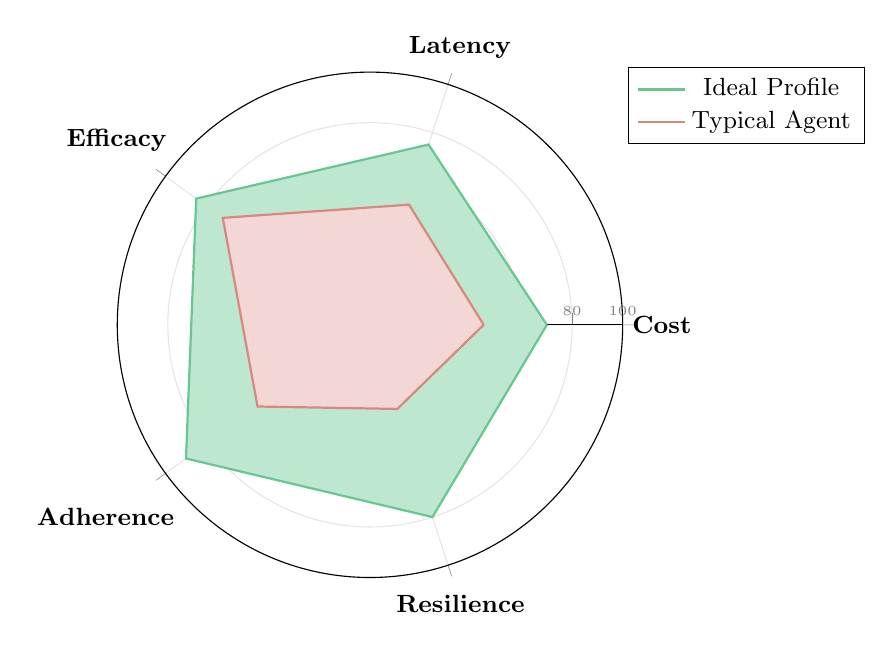
\begin{tikzpicture}
\begin{polaraxis}[
    width=8cm,
    xtick={0, 72, 144, 216, 288},
    xticklabels={Cost, Latency, Efficacy, Adherence, Resilience},
    xticklabel style={font=\small\bfseries},
    ytick={20, 40, 60, 80, 100},
    yticklabels={20, 40, 60, 80, 100},
    yticklabel style={font=\tiny, color=gray},
    ymin=0, ymax=100,
    grid=both,
    grid style={gray!20},
    %title={\textbf{CLEAR Framework Dimensions}},
    %title style={font=\small, text=alchedark, at={(0.5, 1.24)}},
    legend style={at={(1.01, 1.01)}, anchor=north west, font=\small}
]

% Ideal profile
\addplot[fill=pillar2!30, draw=pillar2!70, thick, mark=none] coordinates {
    (0, 70) (72, 75) (144, 85) (216, 90) (288, 80) (360, 70)
};
\addlegendentry{Ideal Profile}

% Typical production agent
\addplot[fill=riskred!20, draw=riskred!60, thick, mark=none] coordinates {
    (0, 45) (72, 50) (144, 72) (216, 55) (288, 35) (360, 45)
};
\addlegendentry{Typical Agent}

\legend{Ideal Profile, Typical Agent}

\end{polaraxis}
\end{tikzpicture}}
\caption{The CLEAR framework radar chart, comparing an ideal agent profile (high scores across all dimensions) against a typical production agent (with notable gaps in Adherence and Resilience).}
\label{fig:clear_radar}
\end{figure}

No single dimension is sufficient. An agent that scores well on accuracy but fails on adherence is not enterprise-ready. An agent that is fast but unreliable is not deployable. The CLEAR framework requires assessment across all five dimensions before deployment.

\subsection{An Evaluation Readiness Maturity Model}

Organizations and research teams operate at widely varying levels of evaluation sophistication. To support structured improvement, we propose an \keyword{Evaluation Readiness Maturity Model} (ERMM) defining five progressive levels of agentic evaluation practice, from basic outcome measurement to continuous risk-weighted assessment. The model is intended as a diagnostic and planning tool, not a compliance checklist---advancing one level provides meaningful improvement regardless of where a team currently sits. Table~\ref{tab:ermm} defines each level.

\begin{table}[htbp]
\centering
\caption{Evaluation Readiness Maturity Model (ERMM): five levels of agentic AI evaluation practice, with characteristics and diagnostic criteria for each level.}
\label{tab:ermm}
\fontsize{6}{6.8}\selectfont
\setlength{\tabcolsep}{2.5pt}
\renewcommand{\arraystretch}{0.92}
\begin{tabularx}{1 \columnwidth}{@{}c l >{\raggedright\arraybackslash}X >{\raggedright\arraybackslash}X@{}}
\toprule
\textbf{Level} & \textbf{Name} & \textbf{Characteristics} & \textbf{Diagnostic Criteria} \\
\midrule
L0 & Outcome-Only & Binary pass/fail and black-box accuracy only & No trajectory logging; single accuracy value \\
L1 & Pillar-Aware & At least two pillars evaluated separately & Tool and model scores separated; no cost reporting \\
L2 & Trajectory-Enabled & Execution traces logged; GPA decomposition applied & Step-level failures diagnosable from traces \\
L3 & Multi-Dimensional & All CLEAR dimensions assessed; CNA tracked & Cost, latency, adherence, and resilience measured \\
L4 & Adaptive & Continuous, risk-weighted evaluation; HITL calibration; horizon tracking & Scenario manifold with risk weights; judge stress tests; refresh cycle \\
\bottomrule
\end{tabularx}
\renewcommand{\arraystretch}{1}
\end{table}

Most published research operates at L0--L1. Most production deployments have not yet reached L2, which requires trajectory instrumentation as a prerequisite. The ERMM is not prescriptive about rate of advancement: moving from L0 to L1 is more impactful for a low-risk workflow than moving from L3 to L4, and organizations should triage by the consequences of evaluation failure in their deployment context. The model's primary value is a shared vocabulary for diagnosing where evaluation gaps exist and a concrete roadmap for closing them.

\subsection{Simulation-Based Testing: Synthetic Users and Multi-Turn Stability}

A significant challenge in agent development is proving readiness for production before the agent encounters real users. Tools like \keyword{ArkSim} have emerged to facilitate multi-turn conversation simulation between agents and synthetic users~\citep{arksim_primary}.

ArkSim, an open-source framework designed for LangChain and LangGraph agents, integrates evaluations into the developer workflow via CI/CD platforms. This allows for the detection of regressions and failures early in the lifecycle. Multi-turn simulation is particularly effective for testing:

\begin{itemize}
    \item \textbf{Context loss during long interactions}: Whether the agent maintains awareness of constraints and information established in early turns.
    \item \textbf{Unexpected conversation paths}: Scenarios that emerge only after several turns of interaction and would not be captured by single-turn evaluation.
    \item \textbf{Idempotency}: The ability of an agent to handle retries safely without causing unintended side effects, such as duplicating a purchase or a data entry.
    \item \textbf{Edge cases in multi-turn reasoning}: Reasoning failures that only emerge when the agent must synthesize information across multiple turns.
\end{itemize}

Simulation-based testing bridges the gap between static benchmarks and production reality. By generating synthetic user interactions that approximate the diversity and unpredictability of real users, simulation enables teams to find issues before users do.

\subsection{Human-in-the-Loop: Calibrating Automated Evaluators for High-Stakes Domains}

Human-in-the-loop (HITL) processes remain essential to audit evaluation results and ensure reliability~\citep{production_ready_agentic}. Humans provide the ground truth labels for ``golden testing datasets'' used to verify agent-generated intents. However, human evaluation at scale is not economically viable for most organizations.

The practical approach is a \keyword{layered evaluation strategy}:

\begin{enumerate}
    \item \textbf{Automated evaluation} for structured, verifiable outputs: Format compliance, factual accuracy against known sources, constraint violation detection.
    \item \textbf{LLM-as-a-Judge} for scalable quality assessment: Reasoning coherence, output quality, decision appropriateness---calibrated against human judgments.
    \item \textbf{Agent-as-a-Judge} for complex, multi-step evaluations: Where fine-grained feedback on specific reasoning steps and tool interactions is required.
    \item \textbf{Human evaluation} for calibration and high-stakes decisions: Periodic review of automated evaluation results, assessment of ambiguous cases, and final approval for high-stakes deployments.
\end{enumerate}

Effective tooling must prioritize the \textbf{``right'' traces for human review}---such as anomaly signals or low-confidence scores---rather than random sampling. Not all traces are equally informative; human attention should be directed toward the cases where automated evaluation is least confident or most surprising.

This layered approach ensures that human expertise is deployed where it adds the most value, while automated methods handle the volume of evaluation that humans cannot.
% ══════════════════════════════════════════════════════════════════════
% SECTION VII
% ══════════════════════════════════════════════════════════════════════
\section{The Evaluation Tooling Landscape: Open Source Packages and Industry Platforms}
\label{sec:tooling}

The methodological frameworks described in the preceding sections require practical tooling to be adopted at scale. Between 2024 and 2026, a rapidly maturing ecosystem of open source packages and industry platforms has emerged to address the evaluation gap. This section surveys the current landscape, organized by function, and identifies the strengths and limitations of each category.

\subsection{Open Source Evaluation and Simulation Packages}

The open source community has been instrumental in advancing agentic evaluation, particularly in areas where proprietary tools lag behind---namely, multi-turn simulation, multi-agent orchestration, and benchmark automation.

\subsubsection{ArkSim (arklexai/arksim)}

ArkSim is an open-source framework designed specifically for multi-turn conversation simulation between agents and synthetic users~\citep{agent_eval_framework}. Built for LangChain and LangGraph agents, it integrates evaluations into the developer workflow via CI/CD pipelines, enabling the detection of regressions and failures early in the development lifecycle.

ArkSim addresses a critical gap in the evaluation landscape: the inability to test agents under realistic multi-turn conditions before deployment. It generates synthetic user personas that interact with the agent across extended conversations, surfacing context loss, idempotency failures, and unexpected conversational paths that only appear after several turns. Key capabilities include:

\begin{itemize}
    \item \textbf{Synthetic user generation}: Configurable personas that simulate diverse user behaviors and edge cases.
    \item \textbf{Multi-turn conversation simulation}: Extended interaction sequences that test context retention and reasoning coherence over time.
    \item \textbf{CI/CD integration}: Automated regression testing that catches failures before they reach production.
    \item \textbf{Idempotency testing}: Verification that agent retries do not cause unintended side effects such as duplicate transactions or data entries.
\end{itemize}

\subsubsection{AgentScope (agentscope-ai/agentscope)}

AgentScope is a production-ready framework with built-in support for multi-agent orchestration and observability~\citep{comprehensive_empirical}. Unlike single-agent evaluation tools, AgentScope is designed to evaluate the behavior of systems where multiple agents interact---surfacing emergent behaviors, coordination failures, and communication inefficiencies that are invisible when each agent is tested in isolation.

The framework provides multi-agent orchestration tools, built-in observability with comprehensive tracing, distributed execution support, and flexible configuration for diverse agent architectures. AgentScope is particularly relevant for organizations deploying multi-agent systems, where the evaluation challenge is qualitatively different from single-agent assessment.

\subsubsection{Evaluation-Agent (Vchitect/Evaluation-Agent)}

The Evaluation-Agent framework, developed by the Vchitect team and recognized with an ACL 2025 Oral and Award, is tailored for evaluating visual generative models using human-like, multi-round strategies~\citep{agent_as_judge_survey}. It represents a domain-specific application of the Agent-as-a-Judge paradigm described in Section~\ref{sec:evaluator}.

Rather than relying on single-pass scoring, the Evaluation-Agent engages in multi-round evaluation---asking follow-up questions, requesting clarifications, and progressively refining its assessment. This mirrors the way human evaluators approach complex judgments, and has been shown to produce evaluations that align more closely with human expert assessments.

\subsubsection{BenchAgents}

BenchAgents automates the creation of evaluation benchmarks using LLM-agent orchestration~\citep{benchagents}. Rather than requiring human experts to manually curate test sets, BenchAgents uses a team of LLM agents to generate, validate, and refine evaluation benchmarks automatically. The framework addresses a fundamental bottleneck in agentic evaluation: the scarcity of high-quality, domain-specific test sets.

\subsection{Industry Platforms and Frameworks}

Alongside open source tools, several industry platforms have emerged that provide managed evaluation infrastructure for enterprise deployments.

\subsubsection{AWS Strands Evals}

AWS Strands Evals provides a practical guide for judgmental evaluation using natural language rubrics and experiments~\citep{strands_evals}. It enables teams to define evaluation criteria in plain English, run structured experiments, and compare agent performance across configurations.

\subsubsection{Amazon Bedrock AgentCore Evaluations}

Amazon Bedrock AgentCore Evaluations provides automated assessment tools for maintaining consistency across contexts~\citep{aws_evaluating_agents}. It is designed for teams deploying agents on the AWS Bedrock platform, and integrates evaluation into the agent development and deployment workflow.

\subsubsection{LangSmith (LangChain)}

LangSmith provides tracing and evaluation templates for LangChain-native workflows~\citep{agent_eval_framework}. As the most widely adopted agent orchestration framework, LangChain's evaluation tooling is particularly important: it provides the infrastructure for capturing execution traces, defining evaluation criteria, and running structured evaluations. LangSmith's tracing capabilities are a practical implementation of the trajectory observability that this paper argues is a prerequisite for meaningful evaluation.

\subsection{Selecting the Right Tooling: A Decision Framework}

The choice of evaluation tooling should be driven by the specific evaluation needs of the organization, not by tool availability. Table~\ref{tab:tool_selection} maps evaluation requirements to tool categories.

\begin{table}[htbp]
\centering
\caption{Evaluation needs mapped to recommended tool categories.}
\label{tab:tool_selection}
\resizebox{0.96\columnwidth}{!}{%
\begin{tabular}{@{}lll@{}}
\toprule
\textbf{Evaluation Need} & \textbf{Tool Category} & \textbf{Example Tools} \\
\midrule
Multi-turn testing & Simulation frameworks & ArkSim \\
Multi-agent evaluation & Orchestration + observability & AgentScope \\
Visual/multimodal eval & Domain-specific judges & Evaluation-Agent \\
Benchmark creation & Automated generators & BenchAgents \\
Enterprise readiness & Managed platforms & Strands Evals \\
Trajectory observability & Tracing frameworks & LangSmith \\
Judge reliability & Perturbation testing & JRH \\
\bottomrule
\end{tabular}
}
\end{table}

No single tool addresses all evaluation needs. Effective evaluation infrastructure typically combines multiple tools---using simulation for pre-deployment testing, tracing for production observability, and judge reliability testing for evaluation quality assurance. The key principle is that evaluation tooling should be selected to match the evaluation methodology, not the other way around.
% ══════════════════════════════════════════════════════════════════════
% SECTION VIII
% ══════════════════════════════════════════════════════════════════════
\section{Future Directions: Closing the Measurement Imbalance}
\label{sec:future}

\subsection{Measuring the Gap: A Cross-Benchmark Coverage Analysis}

The measurement imbalance identified throughout this survey is not only visible in aggregate statistics---it is legible benchmark by benchmark. Table~\ref{tab:benchmark_coverage} maps nine representative benchmarks from the 2024--2026 literature against the four evaluation pillars and three operational dimensions (economic, adherence, resilience) drawn from the CLEAR framework. Ratings reflect the authors' synthesis of published evaluation protocols and should be read as characterizing what each benchmark \emph{explicitly evaluates}, not as an overall quality assessment.

\begin{table*}[htbp]
\centering
\caption{Cross-benchmark coverage analysis. Ratings: $\checkmark$\,=\,explicitly evaluated, $\circ$\,=\,partially or implicitly covered, ---\,=\,not addressed. Assessments are the authors' synthesis based on published evaluation protocols; official benchmark descriptions may differ.}
\label{tab:benchmark_coverage}
\footnotesize
\setlength{\tabcolsep}{4pt}
\resizebox{\textwidth}{!}{%
\begin{tabular}{@{}lccccccc@{}}
\toprule
\textbf{Benchmark} & \textbf{Core Model} & \textbf{Memory} & \textbf{Tool Use} & \textbf{Environment} & \textbf{Economic (Cost/Lat.)} & \textbf{Adherence} & \textbf{Resilience} \\
\midrule
SWE-bench~\citep{beyond_benchmark_islands}    & $\checkmark$ & $\circ$ & $\checkmark$ & $\circ$    & ---        & ---        & ---        \\
WebArena~\citep{beyond_benchmark_islands}     & $\checkmark$ & ---     & $\checkmark$ & $\checkmark$ & ---        & ---        & ---        \\
AgentBench~\citep{comprehensive_empirical}    & $\checkmark$ & ---     & $\checkmark$ & $\checkmark$ & ---        & ---        & ---        \\
GAIA~\citep{beyond_benchmark_islands}         & $\checkmark$ & ---     & $\checkmark$ & $\circ$    & ---        & ---        & ---        \\
$\tau$-bench~\citep{beyond_benchmark_islands} & $\checkmark$ & ---     & $\checkmark$ & $\circ$    & ---        & $\circ$    & ---        \\
HAAF~\citep{beyond_benchmark_islands}         & $\checkmark$ & $\circ$ & $\checkmark$ & $\checkmark$ & $\circ$    & $\checkmark$ & $\circ$    \\
AgentDrive~\citep{beyond_benchmark_islands}   & $\checkmark$ & $\circ$ & $\circ$    & $\checkmark$ & ---        & ---        & $\checkmark$ \\
Agent GPA~\citep{agent_gpa}                   & $\checkmark$ & $\circ$ & $\circ$    & ---        & ---        & ---        & ---        \\
Mind2Web~\citep{beyond_benchmark_islands}     & $\checkmark$ & ---     & $\checkmark$ & $\circ$    & ---        & ---        & ---        \\
\midrule
\textbf{Coverage (\%)} & \textbf{100\%} & \textbf{approx. 33\%} & \textbf{approx. 78\%} & \textbf{approx. 67\%} & \textbf{approx. 11\%} & \textbf{approx. 22\%} & \textbf{approx. 22\%} \\
\bottomrule
\end{tabular}
}
\end{table*}

The pattern is stark. Core Model coverage is universal; Tool Use and Environment are reasonably well-represented. Memory evaluation is partial in only one-third of benchmarks and absent in the rest. Economic, Adherence, and Resilience coverage each falls below 25\% across the set. HAAF is the only benchmark in this survey that explicitly addresses four or more of the seven dimensions. This table is not an argument that every benchmark must cover every dimension; domain-specific benchmarks rightly focus on the dimensions most relevant to their deployment context. It is, however, a concrete illustration of where the research community has concentrated its measurement effort and where the gaps are largest---gaps that Table~\ref{tab:benchmark_coverage} makes difficult to dispute.

\subsection{Integrating Human-Centered and Economic Metrics}

A systematic review of papers from 2023 to 2025 conducted by \citet{measurement_imbalance} reveals a \keyword{measurement imbalance} within that study's review corpus: approximately 83\% of the evaluations analyzed focused primarily on technical performance, while only around 30\% addressed human-centered factors and a similar proportion considered economic impacts. These percentages are specific to the coding and review criteria used by that study and should be interpreted as characterizing a particular sample of the literature, not as universal constants. The directional finding---that technical metrics dominate over human-centered and economic ones---is consistent with the broader pattern visible across the surveyed literature. Figure~\ref{fig:measurement_imbalance} visualizes this imbalance.

\begin{figure}[htbp]
\centering
% Measurement Imbalance in Agentic AI Evaluation
\resizebox{0.68\columnwidth}{!}{%
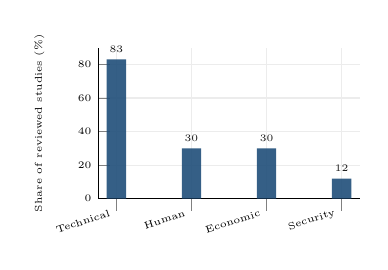
\begin{tikzpicture}
\begin{axis}[
    ybar,
    width=4.9cm,
    height=3.5cm,
    bar width=7pt,
    ymin=0,
    ymax=90,
    ylabel={Share of reviewed studies (\%)},
    ylabel style={font=\tiny, scale=0.72, transform shape, at={(axis description cs:-0.18,0.5)}},
    symbolic x coords={Technical, Human, Economic, Security},
    xtick=data,
    x tick label style={font=\tiny, scale=0.72, transform shape, rotate=18, anchor=east},
    ytick={0,20,40,60,80},
    yticklabel style={font=\tiny, scale=0.72, transform shape},
    nodes near coords,
    nodes near coords style={font=\tiny\bfseries, scale=0.72, transform shape},
    every axis plot/.append style={draw=none, fill opacity=0.9},
    grid=major,
    grid style={gray!15},
    axis lines*=left,
    enlarge x limits=0.08,
    clip=false
]

\addplot[fill=alcheblue] coordinates {
    (Technical, 83)
    (Human, 30)
    (Economic, 30)
    (Security, 12)
};

%\node[font=\scriptsize, text=riskred, align=center] at (axis cs:Security,20)
%    {Technical emphasis remains dominant;\\security coverage is thinnest.};

\end{axis}
\end{tikzpicture}
}
\vspace{-0.2em}
\fontsize{6}{6.8}\selectfont
\caption{The measurement imbalance in agentic AI evaluation. Technical metrics dominate the literature, while security and human-centered considerations remain critically underrepresented.}
\label{fig:measurement_imbalance}
\end{figure}

The measurement imbalance is not merely an academic concern. It has direct business consequences:

\begin{itemize}
    \item Organizations invest in agents that perform well on technical benchmarks but fail to deliver value to users.
    \item Procurement decisions are made based on accuracy metrics that do not account for cost, latency, or reliability.
    \item Agents are deployed that are technically capable but operationally fragile, leading to production incidents and erosion of trust.
\end{itemize}

Closing this imbalance requires three shifts:

\begin{enumerate}
    \item \textbf{Mandatory economic reporting}: Every benchmark result should include CNA or an equivalent cost-normalized metric. Accuracy without cost context is misleading.
    \item \textbf{Human-centered evaluation integration}: User satisfaction, task completion from the user's perspective, and the quality of the human-agent interaction should be standard evaluation dimensions, not afterthoughts.
    \item \textbf{Multi-dimensional deployment criteria}: The CLEAR framework (or equivalent) should be adopted as a standard for deployment readiness, requiring assessment across all five dimensions.
\end{enumerate}

\subsection{The Role of Standardized Web Conduct and Multi-Agent Interaction Protocols}

As agentic AI matures, the industry is moving toward a more nuanced understanding of ``agenticness'' as a spectrum rather than a binary property~\citep{aiagentindex}. Systems are increasingly being designed with a \keyword{flexible thinking budget}---skipping complex orchestrators for reactive tasks and allocating more tokens and time for deep reasoning tasks like supply chain planning.

This evolution creates new evaluation challenges:

\begin{itemize}
    \item \textbf{Multi-agent evaluation}: When multiple agents interact, emergent behaviors can arise that are not predictable from evaluating each agent in isolation. Metrics for coordination, communication efficiency, and collective decision-making are needed.
    \item \textbf{Standardized interaction protocols}: As agents interact with web services, APIs, and each other, standardized protocols for agent conduct are needed---analogous to robots.txt for web crawlers, but for autonomous AI agents.
    \item \textbf{Cross-platform benchmarking}: Current benchmarks are fragmented and non-comparable. Industry-standard evaluation protocols are needed to enable meaningful comparison across agents and platforms.
\end{itemize}

The development of these standards will require collaboration across industry, academia, and regulatory bodies. Organizations that contribute to standardization efforts will have a voice in shaping the evaluation landscape.

\subsection{Toward Verifiable and Trustworthy Autonomous Agents}

Industry practitioners have articulated aspirational targets for enterprise-grade agentic systems---including 95\%+ task accuracy in multi-turn reasoning workflows~\citep{mckinsey_agentic_ai}---though such figures reflect industry planning horizons and marketing commitments rather than academic consensus benchmarks. Whether 95\% represents a meaningful or achievable threshold depends heavily on task definition, evaluation methodology, and deployment context. We cite this figure as an indicator of where the practitioner community is directing investment, not as a validated scientific target. Reaching even a well-defined accuracy target requires closing the measurement imbalance---integrating technical performance, human-centered assessment, and economic efficiency into a coherent evaluation approach.

The methodological building blocks now exist:

\begin{itemize}
    \item \textbf{Trajectory metrics} that evaluate the complete execution path, not just the final output.
    \item \textbf{Agent-as-a-Judge} paradigms that provide scalable, human-aligned evaluation.
    \item \textbf{CNA} and the CLEAR framework that integrate economic and operational dimensions.
    \item \textbf{Simulation-based pre-deployment testing} that surfaces issues before production.
    \item \textbf{The Four-Pillar Model} that decomposes agent assessment into testable components.
    \item \textbf{The HAAF scenario manifold} that weights evaluation by deployment risk.
\end{itemize}

The challenge is adoption. Most teams are still optimizing for the metric they can measure most easily, not the metric that matters most for production.


\subsection{The Evaluation Horizon Problem}

A less-discussed structural challenge for the field is what we term the \keyword{evaluation horizon}---the finite time interval over which a benchmark retains its discriminative validity before degradation through training data contamination.

As agentic models are continuously trained on large, internet-scale corpora, published benchmarks become part of the training distribution over time. A benchmark released in 2024 may appear on forum discussions, code repositories, and synthetic data generators used in post-training runs in 2025 and 2026. The result is that benchmark performance increasingly reflects how much of the benchmark's specific task distribution an agent has been trained on---a confound that worsens with each model generation and is difficult to detect from evaluation scores alone.

We define the evaluation horizon $H(B, \epsilon)$ of benchmark $B$ as the time interval after which the benchmark's discriminative validity---its ability to distinguish better agents from worse ones---drops below threshold $\epsilon$. If $\delta(t)$ denotes the contamination-adjusted discriminative validity of $B$ at time $t$ after release $t_0$:
\begin{equation}
    H(B, \epsilon) = \inf \{ t > t_0 : \delta(t) < \epsilon \}
\end{equation}
For widely-cited, publicly released benchmarks, this horizon may be as short as 6--18 months given the pace of model releases. This framing has direct implications: benchmark maintainers should budget for regular task refresh cycles; research teams should prefer held-out evaluation sets not released publicly; and the community should weight recently-released, unpublished benchmarks more heavily in comparative assessments. The evaluation horizon problem is also a structural argument for simulation-based and generative evaluation methodologies---task distributions that are generated at evaluation time are harder to contaminate than fixed task sets.

% ══════════════════════════════════════════════════════════════════════
% SECTION IX
% ══════════════════════════════════════════════════════════════════════
\section{Conclusion and Strategic Recommendations}
\label{sec:conclusion}

This survey has synthesized the agentic AI evaluation literature of 2024--2026, identifying structural gaps, reviewing proposed frameworks, and critically examining the tooling ecosystem. The key finding is that evaluation methodologies inherited from static NLP are systematically inadequate for the non-deterministic, multi-step, tool-mediated behavior of agentic systems. Task completion is a necessary but insufficient condition for production readiness. The CLEAR dimensions and Cost-Normalized Accuracy proposed here are conceptual synthesis contributions intended to prompt community standardization discussion---not empirically validated instruments ready for direct adoption. Similarly, the Four-Pillar Model and success masking framing are organizational syntheses rather than novel empirical discoveries.

Organizations and researchers must prioritize trajectory-level observability to understand why agents succeed or fail, particularly in multi-turn interactions where compounding errors are common.

The adoption of Agent-as-a-Judge paradigms offers a scalable path to achieving human-level evaluation quality while significantly reducing costs. However, this must be balanced with rigorous stress-testing of those judges using libraries like the Judge Reliability Harness to ensure they are not merely reflecting their own internal biases.

The economic dimension of agency---specifically the trade-off between accuracy and token consumption---must become a central focus of both academic research and enterprise procurement to prevent the explosion of inference bills and the deployment of operationally fragile systems.

\subsection{Strategic Recommendations}

\subsubsection{For Research Teams}

\begin{enumerate}
    \item \textbf{Report CNA alongside accuracy.} Any benchmark result reported without cost normalization is incomplete and potentially misleading.
    \item \textbf{Adopt trajectory-level evaluation.} Move beyond outcome-only metrics to assess the complete execution path.
    \item \textbf{Stress-test your judges.} Implement JRH-style perturbation testing for any LLM-based evaluation pipeline.
    \item \textbf{Close the measurement imbalance.} Integrate human-centered and economic metrics into evaluation frameworks alongside technical performance.
\end{enumerate}

\subsubsection{For Engineering Teams}

\begin{enumerate}
    \item \textbf{Instrument your traces before you instrument your benchmarks.} Trajectory observability is a prerequisite for meaningful evaluation. If you cannot replay the reasoning path for a failed task, you cannot diagnose the failure.
    \item \textbf{Use multi-turn simulation to find issues before users do.} Tools like ArkSim can surface context loss, idempotency failures, and unexpected conversation paths before they appear in production logs.
    \item \textbf{Apply the four pillars selectively by risk.} Not every workflow requires evaluation across all four pillars at equal depth. Triage by consequence: high-stakes workflows warrant full trajectory evaluation; lower-stakes workflows can tolerate lighter-weight assessment.
    \item \textbf{Implement the CLEAR framework for deployment governance.} No agent should be promoted to production without assessment across all five CLEAR dimensions.
\end{enumerate}

\subsubsection{For Leadership and Procurement}

\begin{enumerate}
    \item \textbf{Require multi-dimensional evaluation in vendor assessments.} Accuracy-only benchmarks are insufficient for procurement decisions. Demand CNA, CLEAR assessments, and trajectory-level evaluation results.
    \item \textbf{Budget for evaluation infrastructure.} The cost of inadequate evaluation---production incidents, compliance violations, eroded trust---far exceeds the cost of building proper evaluation infrastructure.
    \item \textbf{Invest in organizational learning.} Evaluation data should inform agent design, deployment decisions, and risk calibration across the organization.
\end{enumerate}

\vspace{1cm}
\noindent By adopting a multi-dimensional approach that spans technical, human-centered, and economic factors, the industry can bridge the gap between impressive laboratory results and reliable, production-grade autonomous infrastructure.

%\vspace{2cm}
%\begin{center}
%\rule{0.3\textwidth}{0.4pt}\\[6pt]
%\textit{\small \textcopyright\ 2026 Alchedata. All rights reserved.}
%\end{center}


% ══════════════════════════════════════════════════════════════════════
% REFERENCES
% ══════════════════════════════════════════════════════════════════════
\bibliographystyle{IEEEtranN}
\bibliography{references}

\begin{IEEEbiographynophoto}{Fei Wang}
Fei Wang is a Cofounder of Alchedata AI, where he leads the development of foundation model post-training infrastructure and multi-agent orchestration systems for enterprise data services. Prior to this, he served as Head of Personalization Science at Amazon Prime Video, where he led a team scientists and engineers building recommendation and search systems at scale, including the StreamFM foundation model for video ranking. Before Amazon, he was Senior Director of AI Research at Visa Research, where he  led the development  of AI-driven fraud detection and recommender systems deployed across Visa's core products. Earlier in his career, he held lead scientist positions at AIBEE, Zepp Health (Amazfit), and AliveCor, where he developed FDA-approved algorithms for cardiovascular disease detection from ECG/PPG signals. He received his Ph.D. in Computer Science from the University of Florida and has authored 80+ publications  and 70+ patents. His research interests include foundation model post-training, reinforcement learning from human feedback, personalization systems, and agentic AI.
\end{IEEEbiographynophoto}

\begin{IEEEbiographynophoto}{Salon Ren}
Salon Ren is a Cofounder of Alchedata AI specializing in multi-agent system design and evaluation methodology. His interests include trajectory-level observability and the operationalization of AI safety frameworks in production environments.
\end{IEEEbiographynophoto}

\begin{IEEEbiographynophoto}{Eric Wang}
Eric Wang is a researcher at Alchedata AI with a focus on enterprise AI deployment, cost optimization, and governance frameworks for autonomous systems. He contributes to the development of practical evaluation standards for agentic AI.
\EOD
\end{IEEEbiographynophoto}

\end{document}

